 %%%   DO NOT EDIT THIS SECTION  %%%

\section{Instrument}
\label{sec:instrument} %3

PICO meets all of its science-derived instrument requirements (Table~\ref{tab:STM})
with a single instrument: an imaging polarimeter with 21 frequency
bands centered between 21 and 799\,GHz. The instrument is built around
a two-reflector Dragone-style telescope
(\S\,\ref{sec:telescope}) with an internal aperture stop between the
primary and secondary. The focal plane is populated by 12,996
transition edge sensor (TES) bolometers (\S\,\ref{sec:focal_plane})
read out using a time-domain multiplexing scheme
(\S\,\ref{sec:detector_readout}). The instrument employs a single
science observing mode: fixed rotation-rate imaging while scanning the
sky.


A V-groove radiator assembly provides passive cooling
(\S\,\ref{sec:radiative_cooling}). The instrument is configured inside
the shadow of the V-grooves, thermally and optically shielded from the
Sun. The sun shadow cone depicted in Fig.~\ref{fig:InstrumentCAD} is
$29\degree$. The angle to the Sun during the survey, $\alpha = 26\degree$
(\S\,\ref{sec:survey_design} and Fig.~\ref{fig:MissionDesignFigure}), is supplemented with a margin of
$3\degree$ to account for the radius of the sun ($0.25\degree$), pointing
control error, design margin, and alignment tolerances.

The V-groove assembly is attached to the bipod struts that support the
instrument structural ring. The ring supports the primary reflector
and telescope box. The telescope box contains the actively cooled
components (\S\,\ref{sec:cadr}, \S\,\ref{sec:4kcooler}), including
the secondary reflector, the focal plane and sub-kelvin adiabatic
refrigerator structures. Just inside the box, a thermal liner serves
as a cold optical baffle and aperture stop.

During the survey, the instrument is spun at 1 rpm
(\S\,\ref{sec:survey_design}). Spacecraft control is simplified by
mounting the instrument on a spinning spacecraft module, while a
larger non-spinning module houses most spacecraft subsystems
(\S\,\ref{sec:spacecraft}). Instrument elements that act as heat
sources are accommodated on the spinning module of the
spacecraft. Instrument integration and test (I\&T) is described in
\S\,\ref{sec:iandt}.



\subsection{Telescope}
\label{sec:telescope} %3.1

PICO telescope design is driven by a combination of science
requirements and physical volume limits. The science requirements are:
a large diffraction-limited field of view (DLFOV) sufficient to
support $\sim10^4$ detectors, arcminute resolution at 800\,GHz, low
spurious polarization, and low sidelobe response. All
requirements are met with PICO's 1.4\,m aperture modified open-Dragone
design. There are no moving parts in the PICO optical system.

The PICO optical design was selected following a trade study examining
cross-Dragone, Gregorian Dragone, and open-Dragone designs
\citep{Young2018}.  The open-Dragone and crossed-Dragone offer more
diffraction-limited focal plane area than the Gregorian Dragone
\citep{deBernardis2018}, and are able to support enough detectors to
provide the required sensitivity. The open-Dragone does not require
the massive and voluminous baffles that the cross-Dragone does, and
and hence can satisfy the aperture size requirement within the shadow
cone.

PICO's initial open-Dragone design has been modified by adding an
aperture stop and adding corrections to the primary and secondary
reflectors to enlarge the DLFOV. The detailed geometric
parameterization of the PICO optical design is described in
\cite{Young2018}. The primary reflector (270\,cm $\times$ 205\,cm) is
passively cooled and the secondary reflector (160\,cm $\times$
158\,cm) is actively cooled. The highest frequency (900\,GHz) sets the
surface accuracy requirement of the reflectors to
$\sim \lambda/14 =24\,\mu{\rm m}$. The focal ratio is 1.42. The
slightly concave focal surface, which has a radius of curvature of
4.55\,m, is telecentric to within $0.12\degree$ across the entire FOV.

An actively cooled circular aperture stop between the primary and
secondary reflectors reduces detector noise and shields the focal
plane from stray radiation. Stray-light analysis of the PICO
open-Dragone design using GRASP confirms that the focal plane is
protected from direct view of the sky, and that spillover past the
primary is suppressed by 80\,dB relative to the main lobe for both
co-pol and cross-pol beams. Detailed baffle design will be performed
during mission formulation.

\begin{figure}
\begin{center}
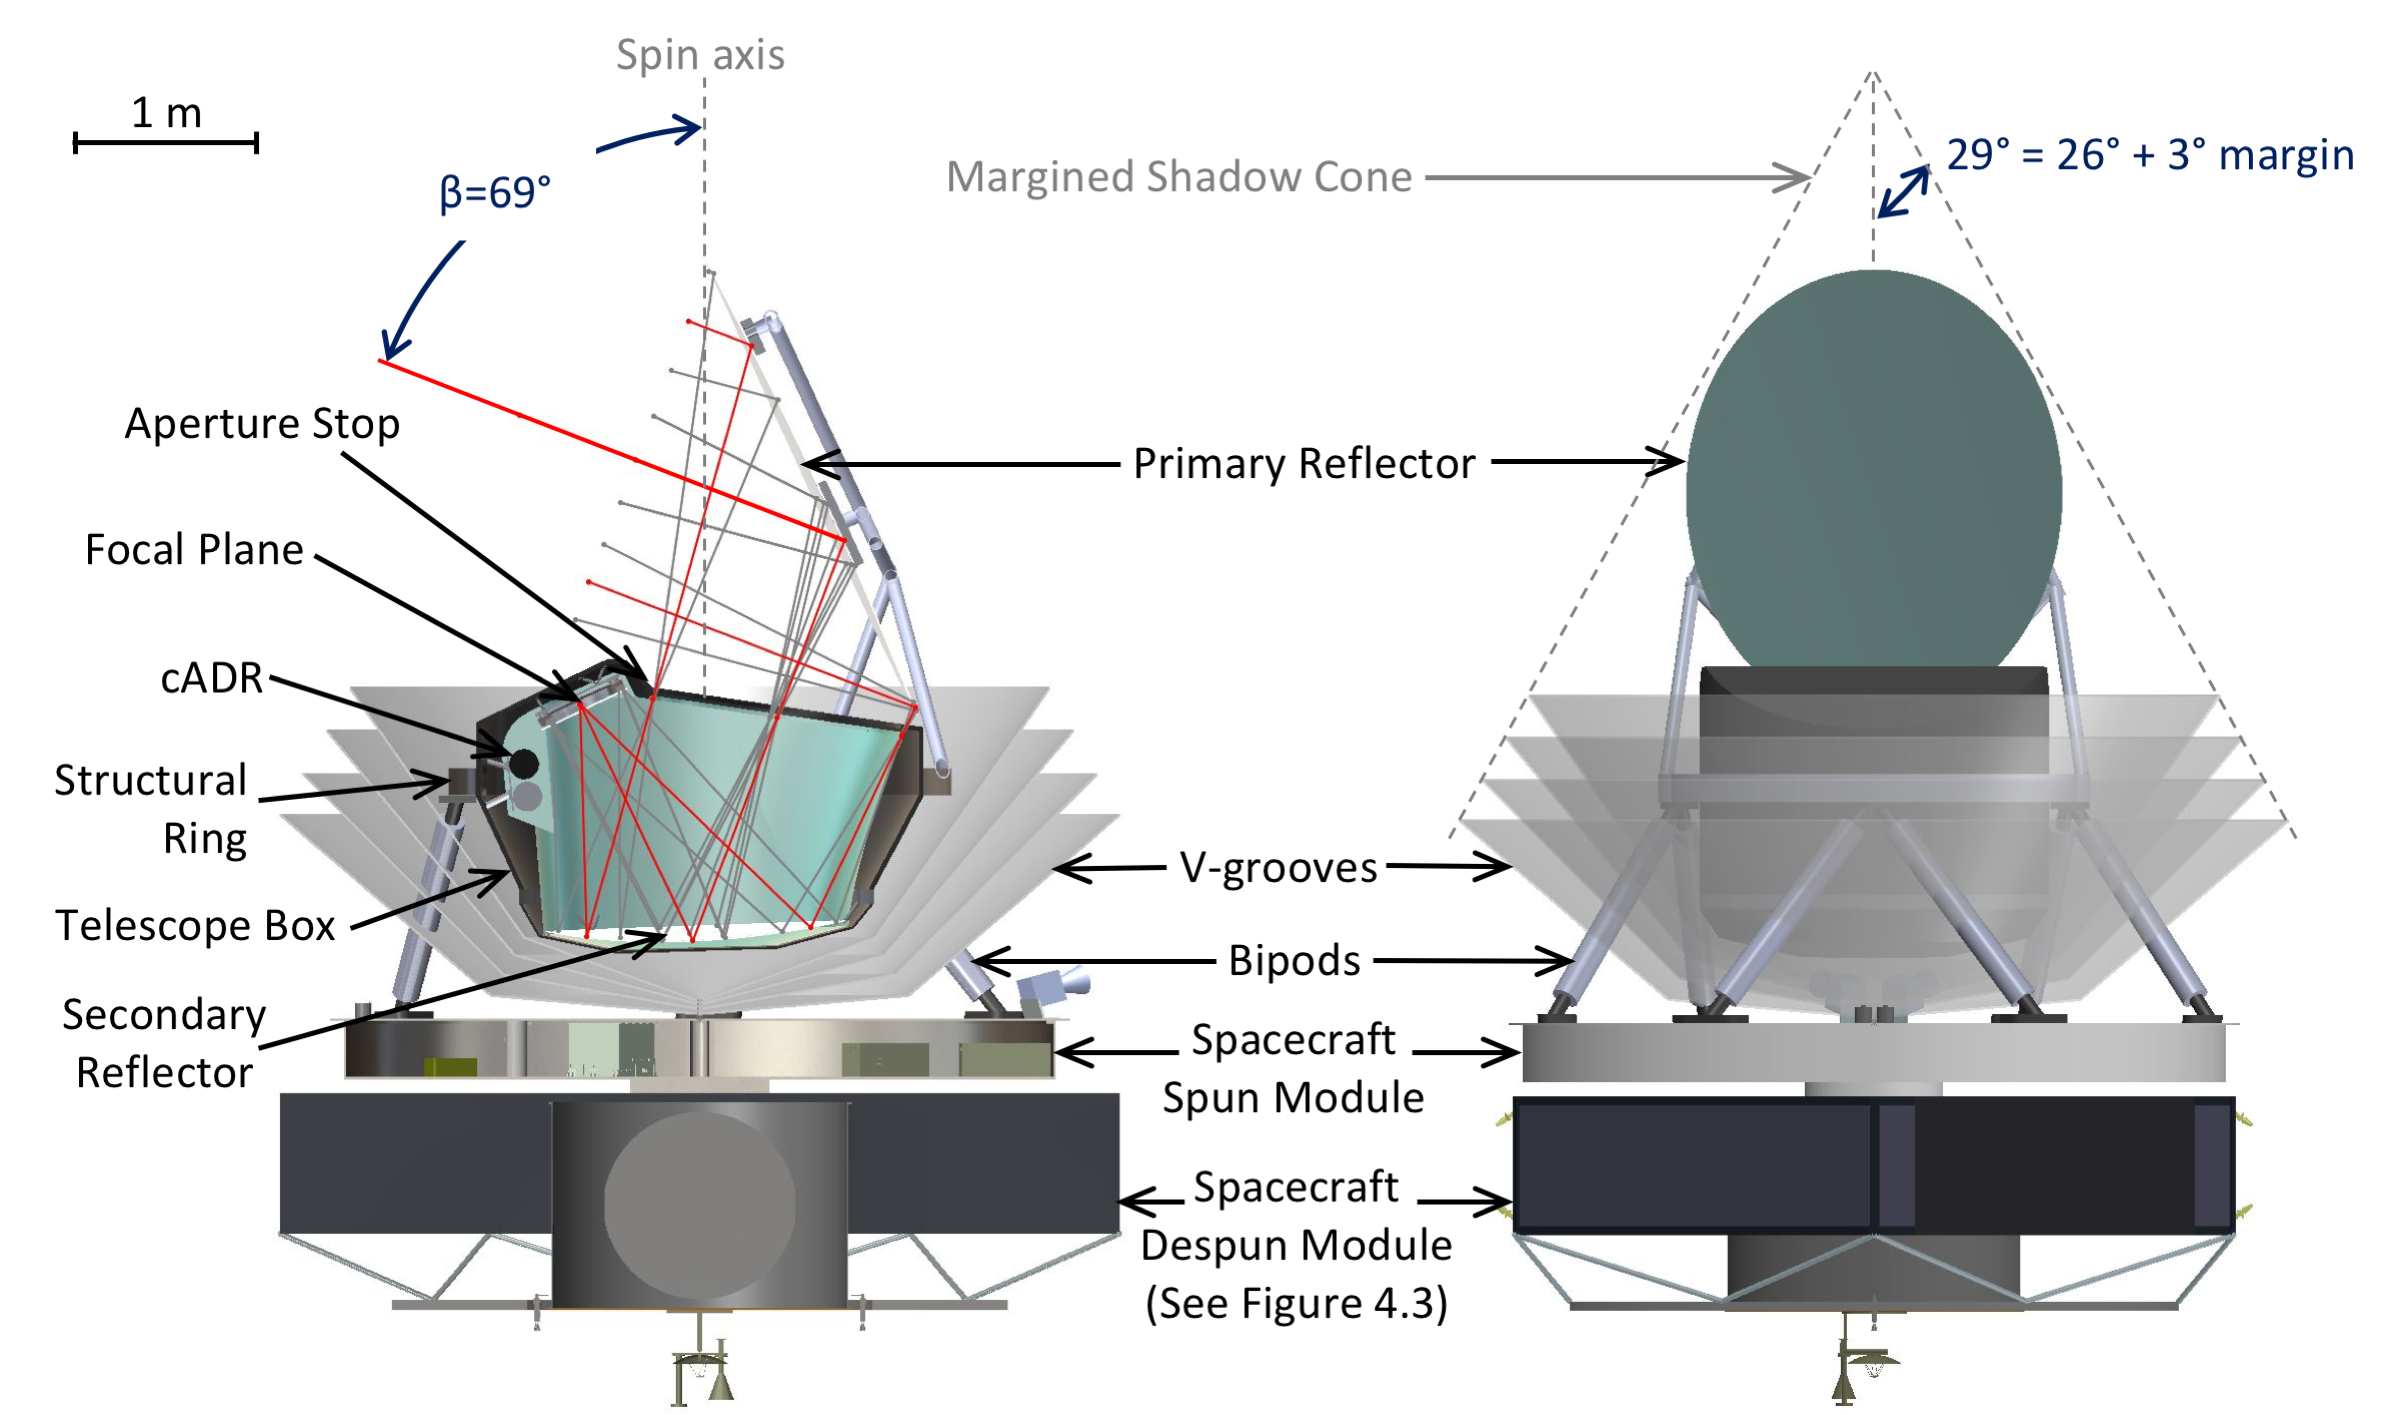
\includegraphics[width=6.25in]{figures/InstrumentCAD.png}
\caption{Detailed PICO instrument configuration. There are no moving or deployed parts. The spacecraft spun module accommodates warm instrument components: the 4\,K cooler compressor and drive electronics, the sub-K cooler drive electronics, and the detector warm readout electronics. {\color{red} Figure to be updated.}\label{fig:InstrumentCAD}}
\end{center}
\end{figure}

% \begin{figure}
% \begin{center}
% 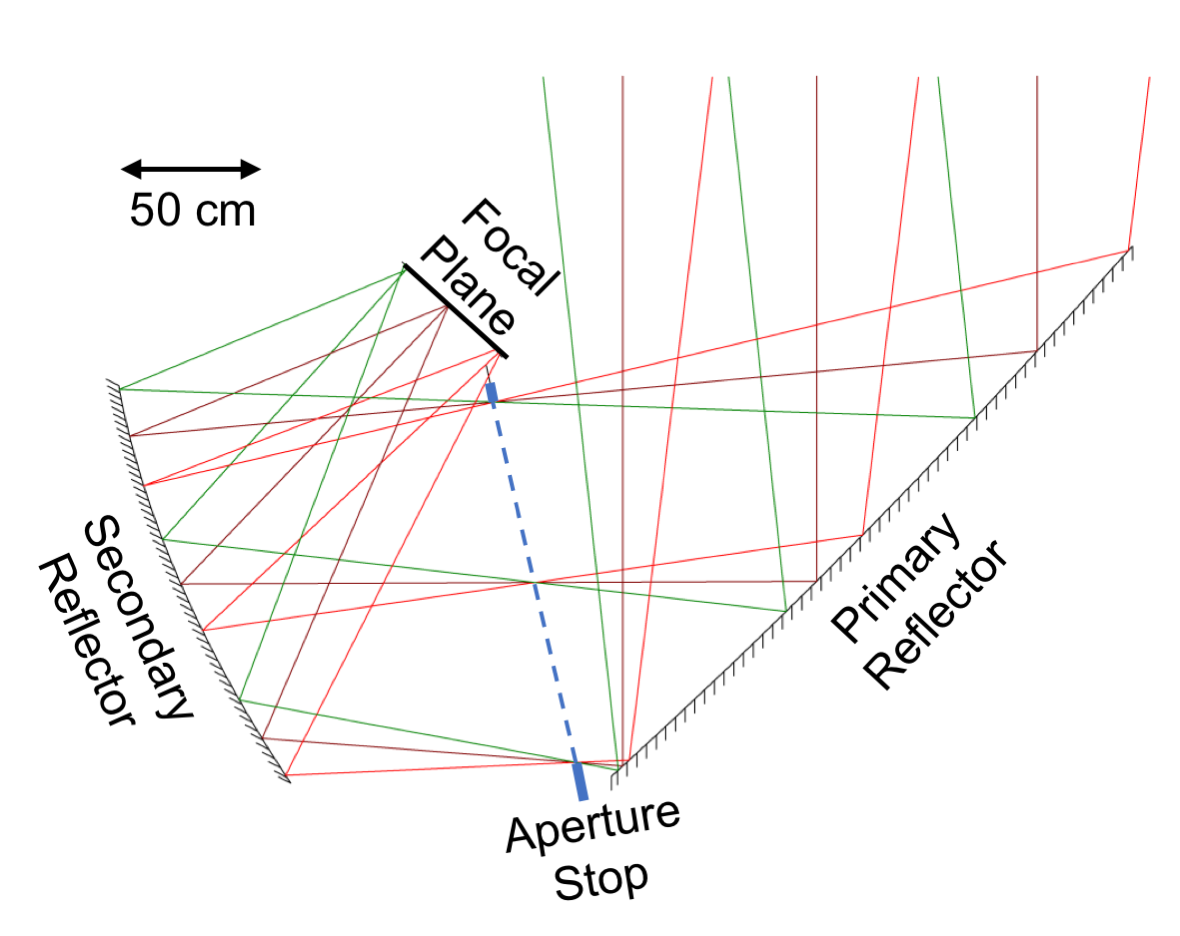
\includegraphics[width=3in]{figures/OpticsDiagram.png}
% \caption{The optical system is compact.\label{fig:OpticsDiagram}}
% \end{center}
% \end{figure}

\begin{figure}
\parbox{3in}{\centering
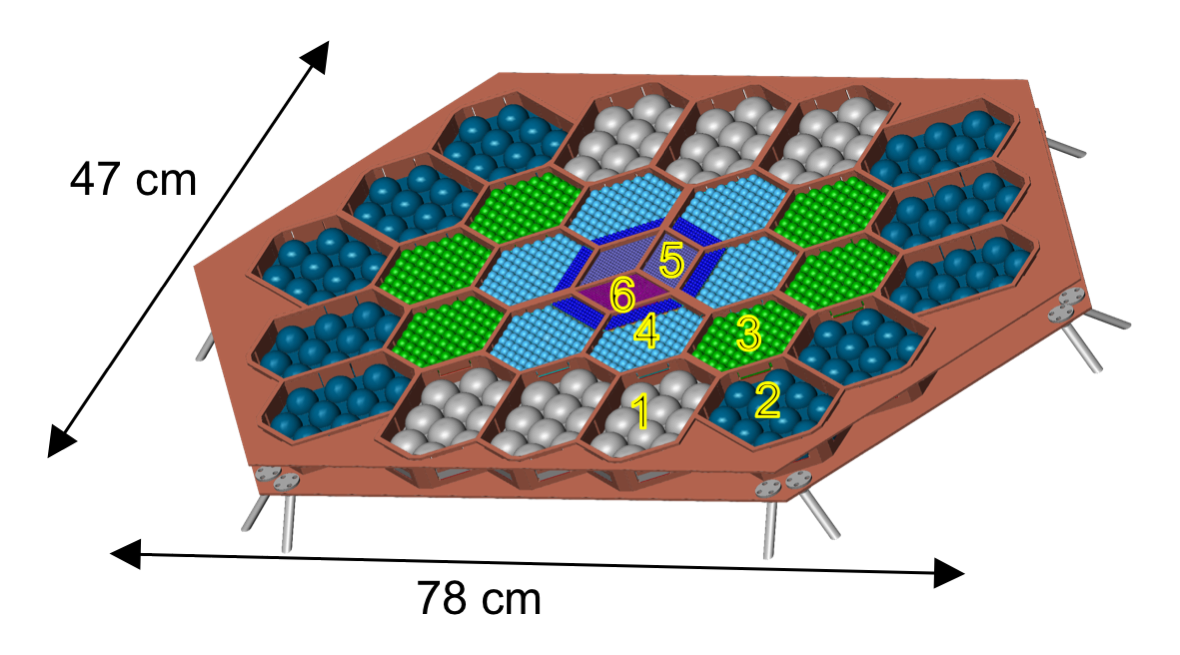
\includegraphics[width=3in]{figures/FocalPlaneMechanical.png}
}
\parbox{3.5in}{\centering
\caption{PICO focal plane. Detectors are fabricated on six types of tiles (shown numbered and colored as in Table~\ref{tab:focal_plane}). The wafers are located on the focal plane such that higher frequency bands, which require better optical performance, are placed nearer to the center.\label{fig:FocalPlaneMechanical}}
}
\end{figure}

\begin{table}
\begin{center}
\caption{PICO makes efficient use of the focal area with multichroic pixels (three bands per pixel, \S\,\ref{sec:low_freq_det}). The sampling rate is based on the smallest beam (Table~\ref{tab:bands}), with 3 samples per FWHM at a scan speed $(360\degree/{\rm min})\sin(\beta=69\degree) = 336\degree/{\rm min}$. {\color{red}Table to be uodated [Tim].} \label{tab:focal_plane}}
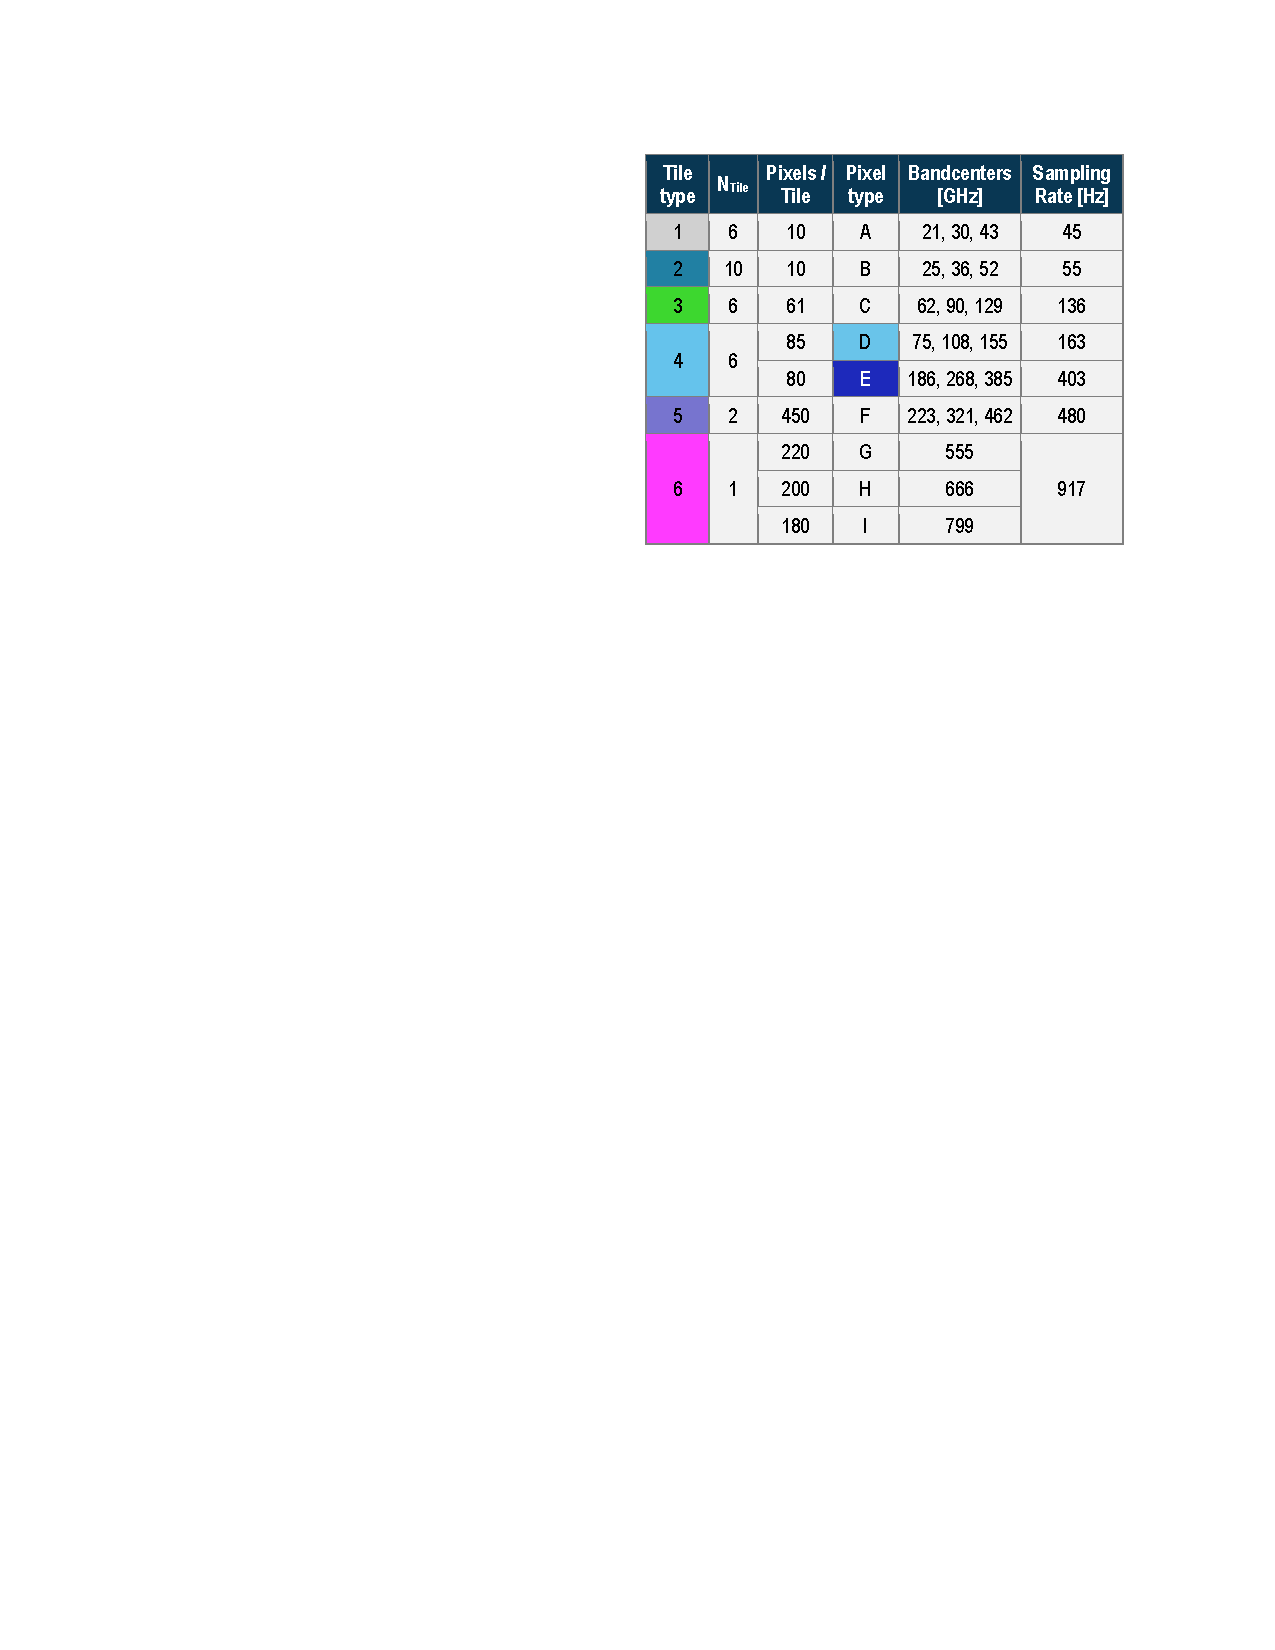
\includegraphics{tables/tab_focal_plane.pdf}
\end{center}
\end{table}

\subsection{Focal plane}
\label{sec:focal_plane} %3.2

PICO's focal plane is populated by an imaging array of transition edge
sensor (TES) bolometers observing in 21 overlapping frequency bands
with 25\% fractional bandwidth and band centers ranging from 21 to
799\,GHz. Polarization is measured by differencing the signals from
pairs of polarization-sensitive bolometers. A conceptual layout of the
PICO focal plane is shown in Fig.~\ref{fig:FocalPlaneMechanical} and
detailed in Table~\ref{tab:focal_plane}.
 
Modern mm/sub-mm detectors are photon-noise limited, so the primary
approach to increase sensitivity is to increase the number of
detectors. The PICO focal plane has 12,996 detectors, 175 times the
number flown on the \textit{Planck} mission, providing a breakthrough
increase in sensitivity with a comparably sized telescope. This
breakthrough is enabled by development and demonstration in suborbital
projects, which now commonly operate arrays of $10^3$--$10^4$ detectors
(\S\,\ref{sec:technology_maturation}).

\subsubsection{21--462\,GHz bands}
\label{sec:low_freq_det} % 3.2.1

The majority of the PICO FOV is populated with multichroic pixels (MCPs)
\citep{Suzuki2014,Datta2014}, which make optimal use of the focal
plane area by feeding three photometric bands from a common broad-band
antenna, with two single-polarization bolometers per band and
therefore six bolometers per pixel.

Several competing optical coupling technologies have matured over the
past ten years using horn-coupling \citep{Duff2016}, antenna-array
coupling \citep{BICEP2015}, and sinuous antenna/lenslet-coupling
\citep{Edwards2012}, delivering quantum efficiency $> 70\,\%$ over more than
an octave of bandwidth. Pixel size, number, and spacing are relatively
agnostic to the coupling scheme, so multiple options are open to PICO
(technology maturation plan described in
\S\,\ref{sec:dev_arrays}). For all of these schemes, niobium
microstrips mediate the signals between the antenna and detectors, and
partition the feed's wide continuous bandwidth into narrow channels
using integrated micro-machined filter circuits \citep{OBrient2013}.

\subsubsection{555--799\,GHz bands}
\label{sec:high_freq_det} % 3.2.2

PICO's highest three frequency channels are beyond the niobium
superconducting band-gap, rendering microstrip filters a poor solution
for defining the optical passband. In this regime, PICO instead
measures a single band with each pixel using feedhorn-coupled
polarization-sensitive bolometers. Radiation is coupled through horns
directly to absorber in the throat of a
waveguide. TES bolometers detect the incident power. 
The waveguide cut-off defines the lower edge of the band,
and quasi-optical metal-mesh filters define the upper edge. Numerous
experiments have successfully used similar approaches
\citep{Shirokoff2011,Bleem2012,Turner2001}. The technology maturation
required for PICO is described in \S\,\ref{sec:dev_arrays}.

\begin{table}[!pt]
\parbox{4.45in}{
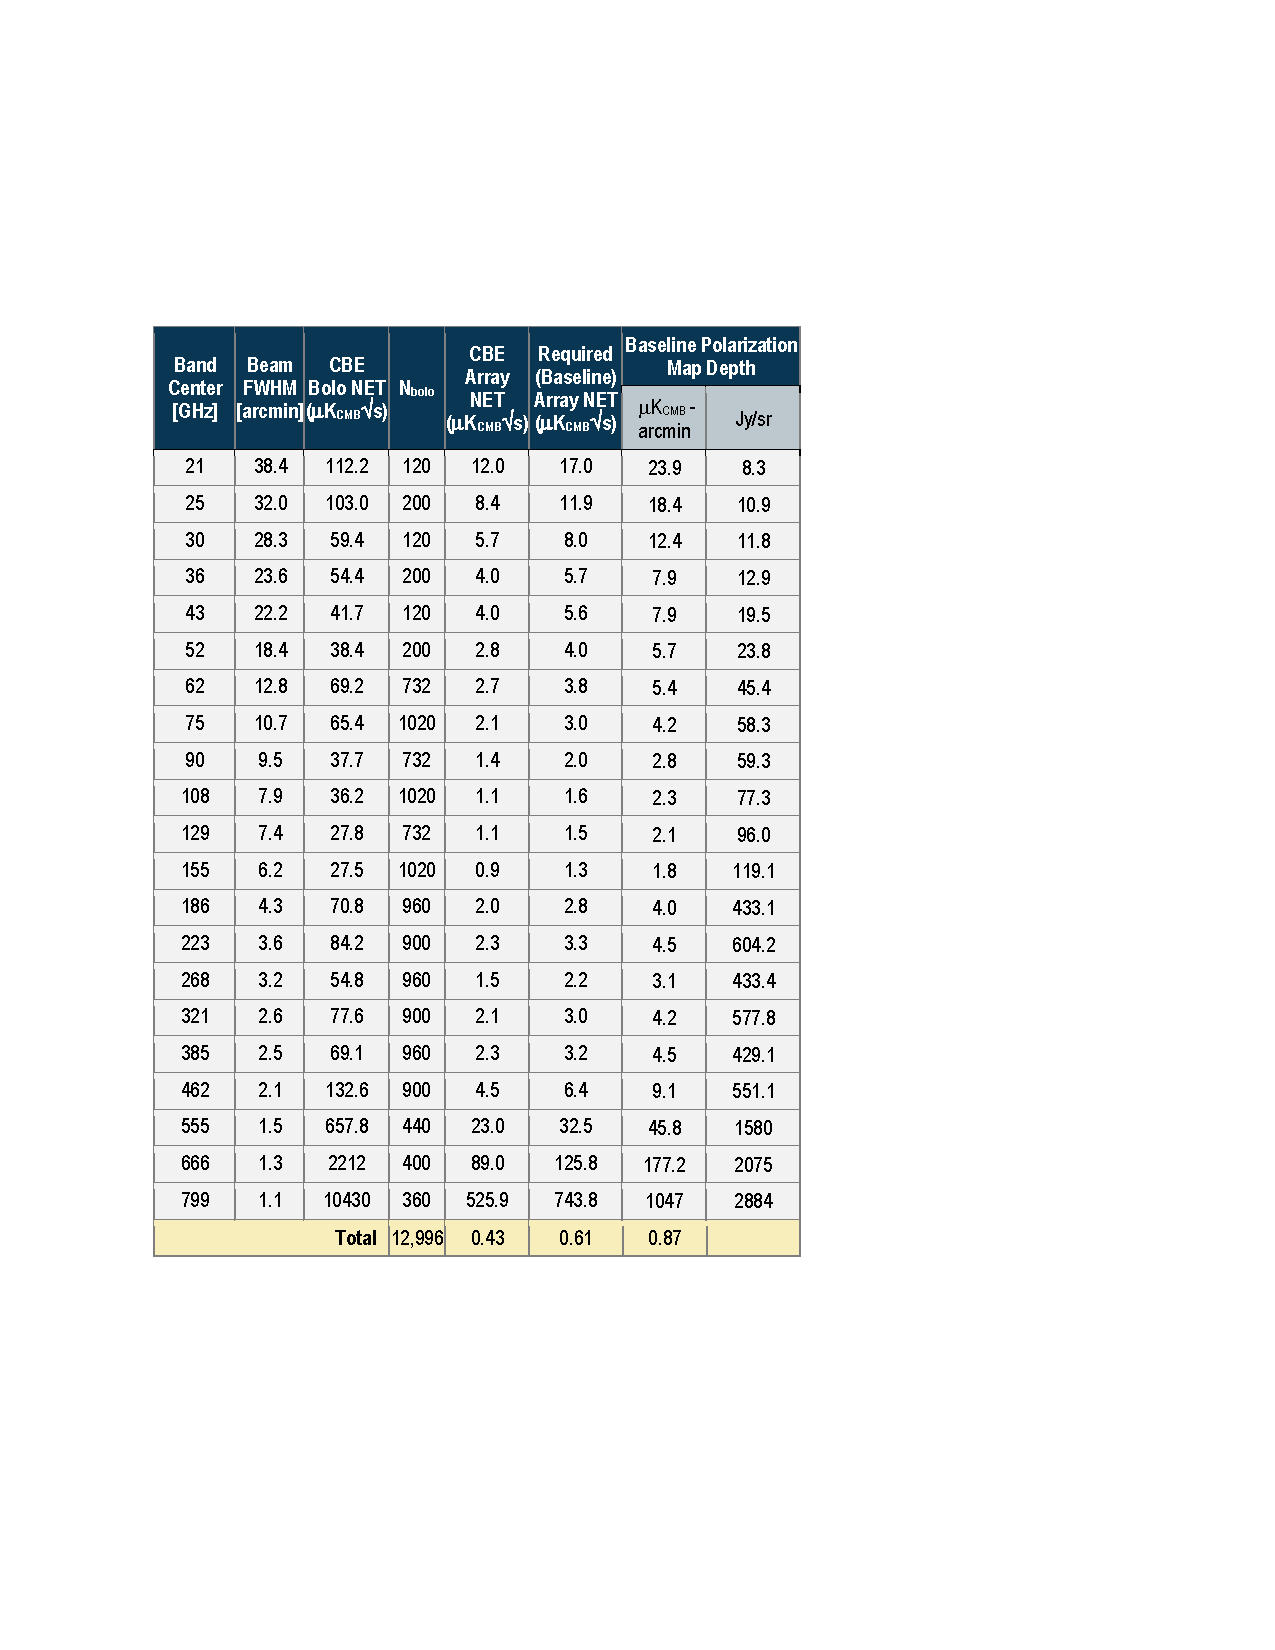
\includegraphics{tables/tab_bands.pdf} }
\parbox{2in}{
\caption{PICO measures in 21 broad overlapping frequency bands with band centers ($\nu_{\rm c}$) from 21\,GHz to 799\,GHz and bandwidth $\Delta\nu/\nu_{\rm c} = 25\,\%$. The beams are single mode, with FWHM sizes of $6.2' \times (155\,{\rm GHz}/\nu_{\rm c})$. The Current Best Estimate (CBE) per-bolometer sensitivity is background limited (\S\,\ref{sec:sensitivity}). The total number of bolometers for each band is equal to (number of tiles) $\times$ (pixels per tile) $\times$ (2 polarizations per pixel), from Table~\ref{tab:focal_plane}. Array sensitivity assumes $90\,\%$ detector operability. The map depth assumes 5\,yr of full sky survey at $95\,\%$ survey efficiency, except the 25 and 30\,GHz frequency bands, which are conservatively excluded during 4\,hr/day Ka-band (26\,GHz) telecom periods (\S\,\ref{sec:ground_segment}).\label{tab:bands}}
}
\end{table}

\subsubsection{Sensitivity}
\label{sec:sensitivity} %3.2.3

PICO's Current Best Estimate (CBE) sensitivity meets the requirements
of the baseline mission with \hbox{$>40\,\%$} margin (Table~\ref{tab:bands}).

We developed an end-to-end noise model of the PICO instrument to
predict full mission sensitivity and provide a
metric by which to evaluate mission design trades. The model considers
four noise sources per bolometer: photon, phonon, TES Johnson, and
readout (from both cold and warm readout electronics). To validate our
calculations, we compared two independent software packages that have
been validated by test on several CMB instruments. The calculations agreed within
1\% both for individual noise terms and for overall mission noise.

Laboratory experiments have demonstrated that TES detectors can be
made background-limited in the low loading environment they would
experience at L2 \citep{Beyer2012}. For PICO, the primary contributor
to noise is the optical load. The sources of optical load are the CMB,
reflectors, aperture stop, and low-pass filters. The CMB and stop
account for the majority of the optical load at all frequencies.  The
CMB gives more than half the load in the middle and upper bands of the
multichroic pixels, but the stop dominates the load in the lowest band
of each pixel.

A detailed description of the PICO noise model and its inputs is
available in \cite{Young2018}. Small differences from
Table~\ref{tab:bands} are due to refinements of the component
temperatures.

The sensitivity model assumes white noise at
all frequencies. Sub-orbital submillimeter experiments have demonstrated TES detectors
that are stable to at least as low as 20\,mHz \citep{Rahlin2014},
meeting the requirements for PICO's scan strategy
(\S\,\ref{sec:survey_design}).

\subsection{Detector readout}
\label{sec:detector_readout} %3.3

Suborbital experiment teams over the past ten years have chosen to use
voltage-biased TESs because their current readout scheme lends itself
to Superconducting Quantum Interface Device (SQUID) based multiplexing. Multiplexing reduces the number of wires
to the cryogenic stages and thus the total thermal load that the
cryocoolers must dissipate. This approach also simplifies the
instrument design.  

In the multiplexing circuitry, SQUIDs function as
low-noise amplifiers and cryogenic switches. The current baseline for
PICO is to use a time-domain multiplexer (TDM), which assigns each
detector's address in a square matrix of simultaneously read columns,
and sequentially cycles through each row of the array
\citep{Henderson2016}. The PICO baseline architecture uses a matrix of
128 rows and 102 columns, requiring some technology maturation
(\S\,\ref{sec:multiplexing}). The thermal loading on
the cold stages from the wire harnesses is subdominant to conductive
loading through the mechanical support structures.  

Because SQUIDs are sensitive magnetometers, suborbital experiments
have developed techniques to shield them from Earth's magnetic field
using highly permeable maetrials and superconducting materials
\citep{Hui2018}.  Total suppression factors better than $10^7$ have
been demonstrated for dynamic magnetic fields \citep{Runyan2010}. PICO
will use these demonstrated techniques to shield SQUID readout chips
from the ambient magnetic environment, which is 20,000 times smaller
than near Earth, as well as from fields generated by on-board
components including the cADR, \S\,\ref{sec:cadr}). In addition, the
cADR is delivered with its own magnetic shielding.

Redundant warm electronics boxes perform detector readout and
instrument housekeeping using commercially available ASICs. The
readout electronics compress the data before delivering it to the
spacecraft. PICO detectors produce a total of 6.1\,Tbits/day assuming
16\,bits/sample, sampling rates from Table~\ref{tab:focal_plane}, and
bolometer counts from Table~\ref{tab:bands}. \textit{Planck} HFI
typically achieved 4.7$\times$ compression in flight with information
loss increasing noise by $\sim10\,\%$
\citep{Pajot2018,PlanckHFI2011}. Suborbital work has demonstrated
6.2$\times$ lossless compression \citep{EBEX2017}. PICO
assumes 4$\times$ lossless compression.

\subsection{Thermal}
\label{sec:thermal} %3.4

Like the \textit{Planck}-HFI instrument, PICO cools its focal plane to
0.1\,K to enable detector operation (\S\,\ref{sec:cadr}). To minimize
detector noise due to instrument thermal radiation, the aperture
stop and reflectors are cooled using both active and radiative cooling
(\S\,\ref{sec:4kcooler}, \S\,\ref{sec:radiative_cooling}, Fig.~\ref{fig:ArchitectureBlockDiagram}).  All
thermal requirements are met with robust margins
(Table~\ref{tab:cooler}).

\begin{table}
\parbox{4.0in}{
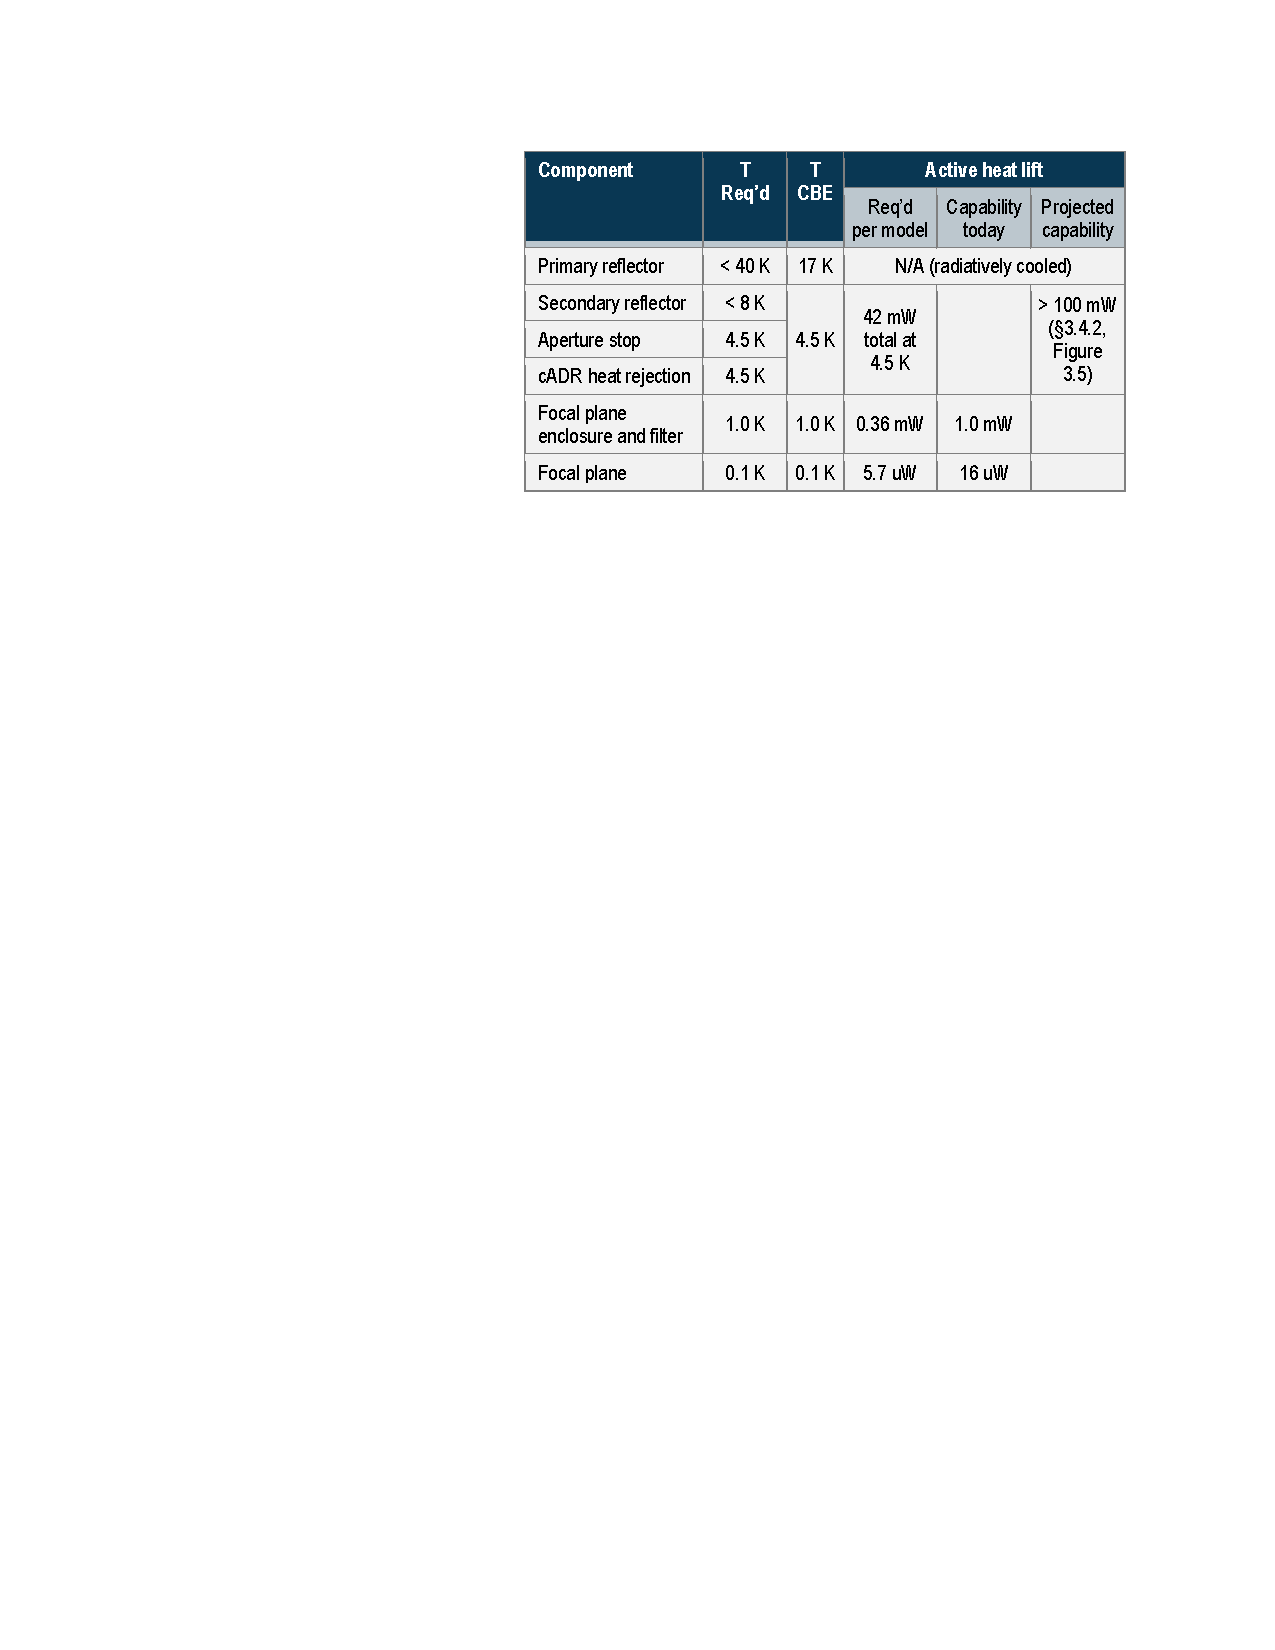
\includegraphics{tables/tab_cooler.pdf} }
\hspace{0.1in}
\parbox{2.5in}{
\caption{Projected cooler heat lift capabilities offer $>100\,\%$ heat lift margin, complying with community best practices \citep{Donabedian2003}. The cADR lift capability at 1\,K and 0.1\,K is from a Goddard quote. Both NGAS and Ball project $>100$\,mW lift capability at $4.5\,$K using higher compression-ratio compressors currently in development (\S\,\ref{sec:4kcooler}). The required loads were calculated using Thermal Desktop. Reference \citep{Ross2004} was used to estimate the thermal conductive loads through mechanical supports. In addition to the listed components, the total 4.5\,K heat load includes the intercept on the focal plane mechanical supports.\label{tab:cooler}} }
\end{table}

\begin{figure}[ht]
\parbox{4.0in}{
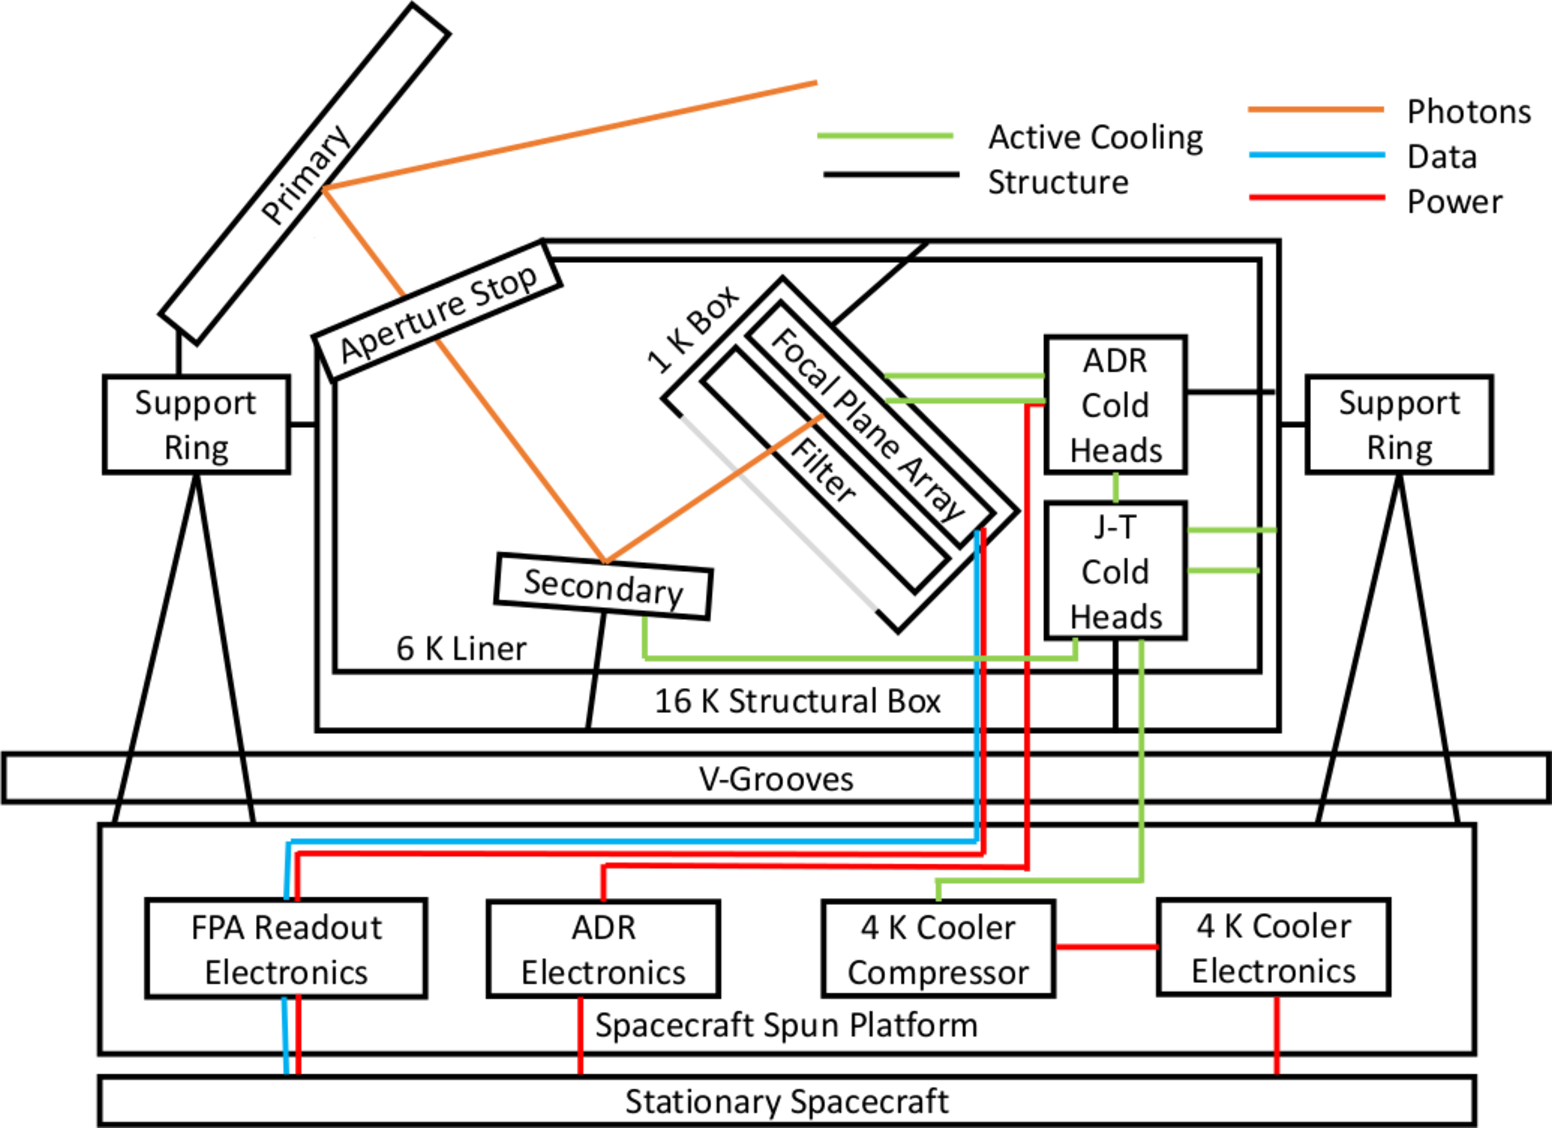
\includegraphics[width=4.0in]{images/ArchitectureBlockDiagram.pdf} }
\hspace{0.05in}
\parbox{2.45in}{
\caption{PICO instrument block diagram. Active coolers provide cooling
  to the 100\,mK focal plane, the surrounding 1\,K box, the 4.5\,K secondary reflector, and the
  4.5\,K thermal liner that acts as a cold aperture stop. Data from the focal
  plane flows to (redundant, cross-strapped) warm readout electronics
  on the spun module of the spacecraft
  bus.\label{fig:ArchitectureBlockDiagram} }  }
\end{figure}


\subsubsection{cADR sub-kelvin cooling}
\label{sec:cadr} %3.4.1

A multi-stage continuous Adiabatic Demagnetization Refrigerator (cADR)
cools the PICO focal plane to 0.1\,K and the surrounding enclosure,
filter, and readout components to 1\,K. The cADR employs three
refrigerant assemblies operating sequentially to absorb heat from the
focal plane at 0.1\,K and reject it to 1\,K. Additionally, the cADR
employs two assemblies operating sequentially to absorb this rejected
heat at 1\,K, cool other components to 1\,K, and reject heat at
4.5\,K. This configuration provides continuous cooling with small
temperature variations at both the 0.1\,K and 1\,K. Heat straps
connect the two cADR cold sinks to multiple points on the focal plane
assembly, which has high thermal conductance paths built in, to
provide spatial temperature uniformity and stability during
operation.The detector arrays are thermally sunk to the mounting frame.  Heat loads in the range of 20\,$\mu$W at 0.1\,K and 1\,mW
at 1\,K (time-average) are within the capabilities of current cADRs
developed by GSFC \citep{Shirron2012,Shirron2016}. The PICO sub-kelvin
loads are estimated at less than half of this capability.

\subsubsection{4 K Cooler}
\label{sec:4kcooler} %3.4.2

A cryocooler system similar to that used on JWST to cool the MIRI
detectors \citep{Durand2008,Rabb2013} removes the heat rejected from
the cADR and cools the aperture stop and secondary reflector to
4.5\,K. Both NGAS (which provided the MIRI coolers) and Ball Aerospace
have developed such coolers under the NASA-sponsored Advanced
Cryocooler Technology Development Program \citep{Glaister2006}. NGAS
and Ball use slightly different but functionally-equivalent hardware
approaches. A 3-stage precooler (acoustic Stirling by NGAS or
mechanical Stirling by Ball) provides $\sim16$\,K precooling to a
separate circulated-gas loop driven by a similar compressor modified
for DC flow. The circulated-gas loop utilizes Joule--Thomson (J-T)
expansion, further cooling the gas to 4.5\,K. The entire precooler
assembly and the J-T circulator compressor are located on the warm
spacecraft, with relatively short tubing lengths conducting the gas
flow from the precooling point to the J-T expansion point. All waste
heat rejected by the cooler compressors and drive electronics is
transferred to the spacecraft heat rejection system. Unlike JWST, the
PICO cooler does not require deployment of the remote cold head.

The J-T expansion point is located close to the cADR heat rejection
point, thereby providing the lowest temperature to the
cADR. Subsequent to cooling the cADR, the gas flow intercepts
conducted heat to the focal plane enclosure, then cools the aperture
stop and the secondary reflector before returning in counterflow to
the circulation compressor.  Model-based projections indicate that the
coolers delivered for MIRI could meet the PICO 4.5\,K heat lift
requirement with $>100\,\%$ margin with minimal changes: the replacement
of the $^4$He gas used for MIRI with $^3$He, plus resizing of the gas
counterflow heat exchangers to take advantage of the $^3$He properties.

\begin{figure}
\parbox{3.5in}{\centering 
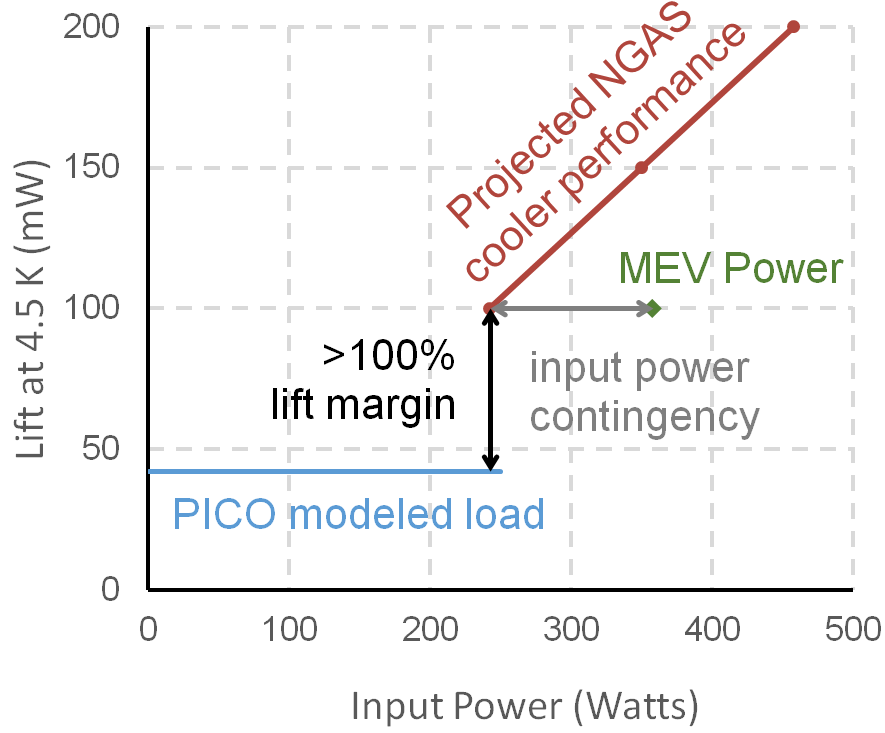
\includegraphics[width=3in]{figures/CoolerFigure.png} }
\parbox{3.0in}{
\caption{Projected performance of the NGAS cooler using a multi-stage
  compressor and $^4$He \citep{Rabb2013} meets PICO's requirements
  with $>100\,\%$ margin. PICO conservatively carries additional input
  power contingency on the efficiency of the
  cooler.\label{fig:CoolerFigure}} }
\end{figure}

It is highly likely that a better solution will be available before
Phase~A. NGAS and Ball are actively working on increasing the flow
rate and compression ratio of the J-T compressor, which should result
in significantly higher system efficiency, and in greater heat-lift
margin above the PICO requirement. These improvements entail the
implementation of well-known techniques (standard thermal
engineering). The NGAS multi-stage J-T compressor has completed
PDR-level development, and is expected to reach CDR level well before
needed for PICO. Projected performance is shown in Fig.~\ref{fig:CoolerFigure}. The
Ball approach started with a larger compressor, required less
modification to achieve comparable performance, and eliminated the
cold bypass-precooling valve that was problematic for MIRI. The Ball
approach uses $^3$He, while the NGAS approach uses $^4$He. Both employ
re-optimized gas heat exchangers (trivial engineering changes).


\subsubsection{Radiative cooling}
\label{sec:radiative_cooling} %3.4.3

A set of four V-groove radiators provides passive cooling. The
outermost of the four V-groove shields shadows the interior shields
from the Sun. The V-grooves radiate to space, each reaching
successively cooler temperatures. The V-groove assembly is
mechanically supported from the spacecraft bus by attachment to the
low-conductance bipod struts that also carry the mechanical loads of
the structural ring (Fig.~\ref{fig:InstrumentCAD}). The V-groove
assembly provides a cold radiative environment to the primary
reflector, structural ring, and telescope box, so radiative loads on
those elements are smaller than the conductive loads through the
mechanical support structures.


\subsection{Instrument integration and test}
\label{sec:iandt} % 3.5

PICO instrument I\&T planning benefits greatly from heritage
experience with the \textit{Planck} HFI instrument \citep{ Pajot2010}.

PICO screens detector wafer performance prior to selection of
flight wafers and focal plane integration. The cADR and 4\,K
cryocooler are qualified prior to delivery. The relative alignment
of the two reflectors under thermal contraction is
photogrammetrically verified in a thermal vacuum (TVAC) chamber.

PICO integrates the flight focal plane assembly and flight cADR in
a dedicated sub-kelvin cryogenic testbed. Noise, responsivity, and focal-plane
temperature stability are characterized using a representative
optical load for each frequency band (temperature-controlled
blackbody). Polarimetric and spectroscopic calibration are
performed.

The focal plane is integrated with the reflectors and structures, and
alignment verified photogrammetrically at cold temperatures in a TVAC
chamber.  The completely integrated observatory (instrument and
spacecraft bus) is tested in TVAC to measure parasitic optical loading
from the instrument, noise, microphonics, and radio-frequency
interference (RFI). The observatory is 4.5\,m in diameter and 6.1\,m
tall, with no deployables.

\newpage
\section{Design reference mission}
\label{sec:design_reference} %4
The PICO design reference mission is summarized in Table~\ref{tab:mission_parameters}.

\subsection{Concept of operations}
\label{sec:operations} %4.1

The PICO concept of operations is similar to that of the successful
\textit{WMAP} \citep{Bennett2003} and \textit{Planck} \citep{Tauber2010} missions. After launch,
PICO cruises to a quasi-halo orbit around the Earth--Sun L2 Lagrange point
(\S\,\ref{sec:mission_design}). A two-week decontamination period is followed by
instrument cooldown, lasting about two months. After in-orbit checkout is complete, PICO begins
the science survey.

PICO has a single science observing mode, surveying the sky
continuously for 5 years using a pre-planned repetitive survey pattern
(\S\,\ref{sec:survey_design}). Instrument data are compressed and stored on-board, then
returned to Earth in daily 4-hr Ka-band science downlink passes
(concurrent with science observations). Because PICO is observing
relatively static Galactic, extragalactic, and cosmological targets,
there are no requirements for time-critical observations or data
latency. Presently, there are no plans for targets of opportunity or
guest observer programs during the prime mission. The PICO instrument
does not require cryogenic consumables (as the \textit{Planck} mission did),
permitting consideration of significant mission extension beyond the prime
mission.

\begin{table}
\centering
\caption{PICO carries margin on key mission parameters. Maximum Expected Value (MEV) includes contingency.}\label{tab:mission_parameters}
\scriptsize\rmfamily
\begin{tabular}{lp{1.5in}}
\hline\noalign{\vskip3pt}
Orbit type&Sun-Earth L2 Quasi-Halo\\
Mission class&Class B\\
Mission duration&5 years\\
Propellant (hydrazine)&213\,kg (77\% tank fill)\\
Launch mass (MEV)&2147\,kg (3195\,kg capability)\\
Max power (MEV)&1320\,W (XX\% of available area)\\
Onboard data storage&4.6\,Tb (3 days of compressed data, enabling retransmission)\\
Survey implementation&Instrument on spin table\\
Attitude control&Zero-momentum 3-axis stabilized\\
\noalign{\vskip3pt}\hline
\end{tabular}
\end{table}

\begin{figure}[!b]
  \begin{minipage}[b]{0.29\textwidth}
    \begin{center}
    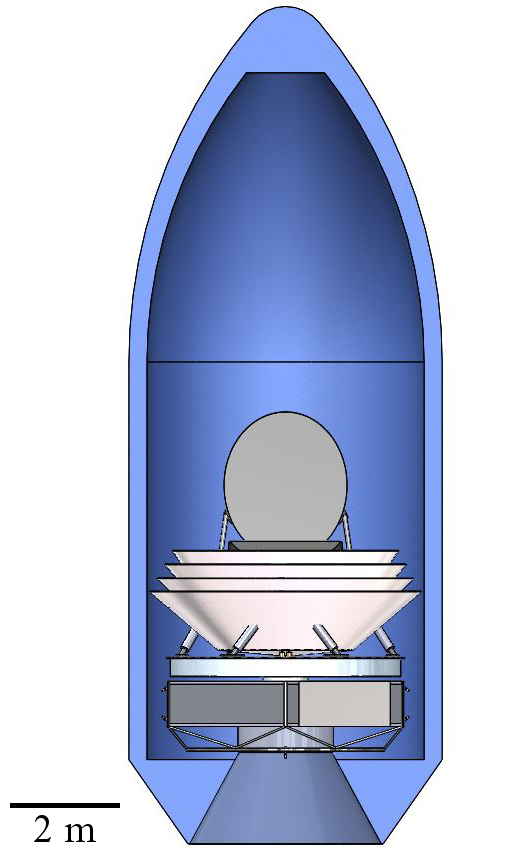
\includegraphics[width=1.1in]{figures/InFairing.JPG}
\caption{PICO is compatible with the Falcon~9.\label{fig:InFairing}}
    \end{center}
  \end{minipage}
%
\begin{minipage}[b]{0.7\textwidth}
    \begin{center}
    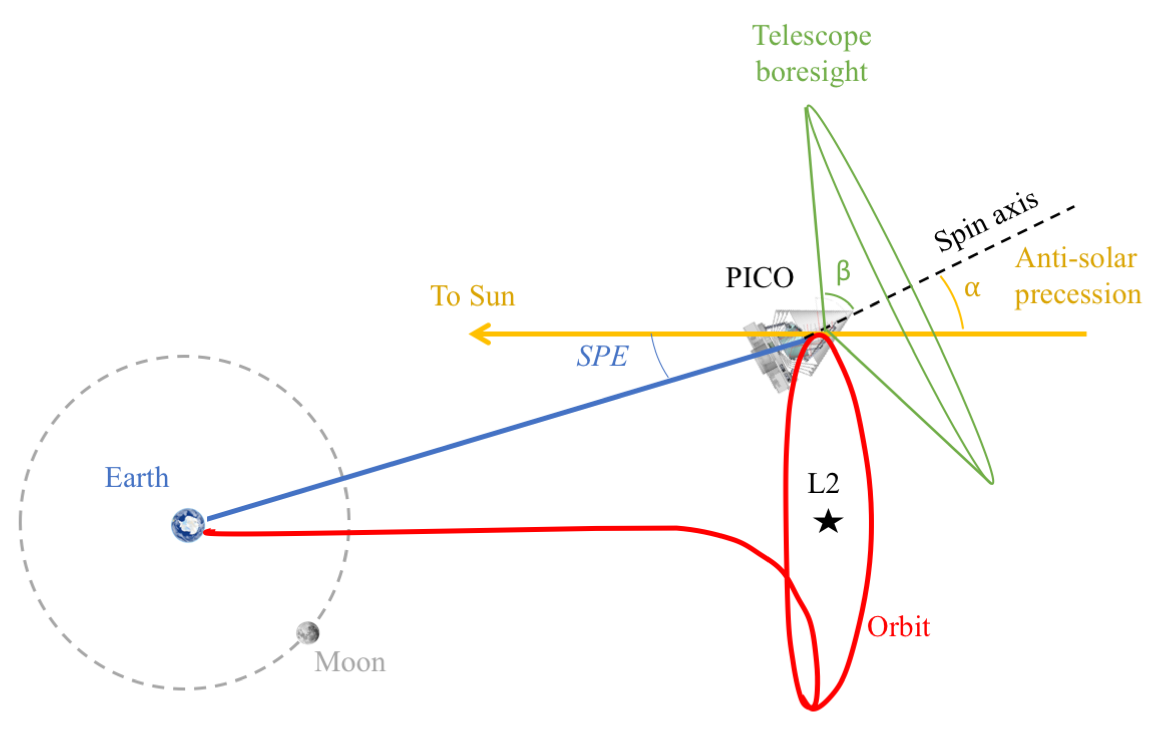
\includegraphics[width=4in]{figures/MissionDesignFigure.png}
\caption{PICO surveys by continuously spinning the instrument about a
  precessing axis.\label{fig:MissionDesignFigure}}
   \end{center}
  \end{minipage}
 
\end{figure}

% \begin{figure}
% \begin{center}
% 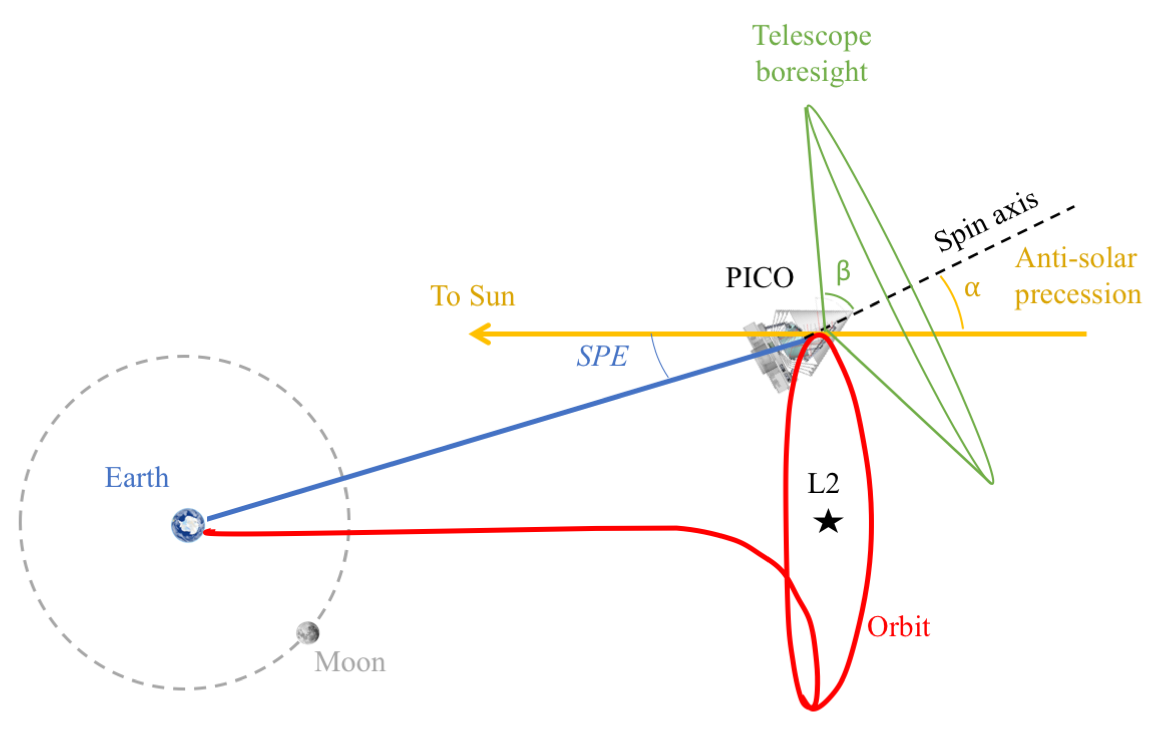
\includegraphics[width=3in]{figures/MissionDesignFigure.png}
% \caption{PICO surveys by continuously spinning the instrument about a
%   precessing axis.\label{fig:MissionDesignFigure}}
% \end{center}
% \end{figure}


% \begin{figure}
% \begin{center}
% 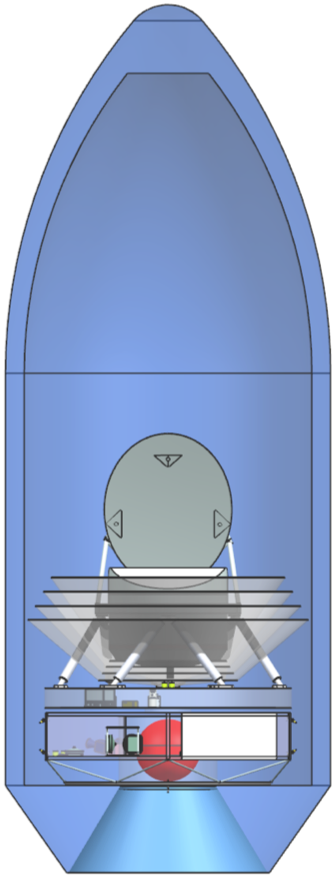
\includegraphics[width=1in]{figures/InFairing.png}
% \caption{PICO is compatible with the Falcon~9.\label{fig:InFairing}}
% \end{center}
% \end{figure}

\subsubsection{Mission design and launch}
\label{sec:mission_design} %4.1.1

PICO performs its science survey from a quasi-halo orbit around the
Earth--Sun L2 Lagrange point. Predecessor missions \textit{Planck} and
\textit{WMAP} both operated in L2 orbits.

L2 orbits provide favorable survey geometry (relative to Earth orbits)
by mitigating viewing restrictions imposed by terrestrial and lunar
stray light. The PICO orbit around L2 is small enough to ensure than
the Sun--Probe--Earth (SPE) angle is less than $15\degree$. This
maintains the telescope boresight $>70\degree$ away from the Earth
(Fig.~\ref{fig:MissionDesignFigure},
$70\degree = 180\degree -\alpha - \beta - \rm{SPE}$). 

High data rate downlink to the Deep Space Network (DSN) is available
from L2 using near-Earth Ka bands. L2 provides a stable thermal
environment, simplifying thermal control. The PICO orbit exhibits no
post-launch eclipses.
 
NASA requires that Probes be compatible with an Evolved Expendable
Launch Vehicle (EELV). For the purpose of this study, the Falcon~9
\citep{SpaceX2015} is used as the reference
vehicle. Figure~\ref{fig:InFairing} shows PICO configured for launch
in a Falcon~9 fairing. The Falcon~9 launch capability for ocean
recovery exceeds PICO's total launch mass (including contingency) by a
$\sim 50\,\%$ margin.

Insertion to the halo manifold and associated trajectory correction
maneuvers (TCMs) require 150\,m\,s$^{-1}$ of total $\Delta V$ by the
spacecraft. The orbital period is $\sim6$\,months. Orbit maintenance
requires minimal propellant (statistical
$\Delta V\sim 2$\,m\,s$^{-1}$\,year$^{-1}$). There are no disposal
requirements for L2 orbits, but spacecraft are customarily
decommissioned to heliocentric orbit.


\subsubsection{Survey design}
\label{sec:survey_design} %4.1.2
 
PICO employs a highly repetitive scan strategy to map the full
sky. During the survey, PICO spins with a period
$T_{\rm spin} = 1$\,min about a spin axis oriented $\alpha=26\degree$
from the anti-solar direction (Fig.~\ref{fig:MissionDesignFigure}). This spin axis
is forced to precess about the anti-solar direction with a period
$T_{\rm prec}= 10$\,hr. The telescope boresight is oriented at an
angle $\beta=69\degree$ away from the spin axis. This $\beta$ angle is
chosen such that $\alpha + \beta > 90\degree$, enabling mapping of all
ecliptic latitudes. The precession axis tracks with the Earth in its
yearly orbit around the Sun, so this scan strategy maps the full sky
(all ecliptic longitudes) within 6 months.

PICO's $\alpha=26\degree$ is chosen to be substantially larger than
the \textit{Planck} mission's $\alpha$ angle ($7.5\degree$) to
mitigate systematic effects by scanning across each sky pixel with a
greater diversity of orientations \citep{Hu2003}. Increasing $\alpha$
further would decrease the sun-shadowed volume available for the
optics and consequently reduce the telescope aperture size. A
deployable sun shade was considered but found not to be required, and
was thus excluded in favor of a more conservative and less costly
approach.

The instrument spin rate, selected through a trade study, matches that
of the \textit{Planck} mission. The study balanced low-frequency
($1/f$) noise subtraction (improves with spin rate) against
implementation cost and heritage, pointing reconstruction ability
(anti-correlated with spin rate), and data volume (linearly correlated
with spin rate).  The CMB dipole appears in the PICO data timestream
at the spin frequency (1\,rpm = 16.7\,mHz). Higher multipole signals
appear at harmonics of the spin frequency starting at 33\,mHz, above
the knee in the detector low-frequency noise
(\S\,\ref{sec:sensitivity}). A destriping mapmaker applied in data
post-processing effectively operates as a high-pass filter, as
demonstrated by \textit{Planck} \citep{Kurki-Suonio2009} (see \S\,\ref{sec:?}). PICO's spin
axis precession frequency is $>400\times$ faster than that of
\textit{Planck}, greatly reducing the effects of any residual $1/f$
noise by spreading the effects more isotropically across pixels.

\subsection{Ground segment}
\label{sec:ground_segment} %4.2

The PICO Mission Operations System (MOS) and Ground Data System (GDS)
can be built with extensive reuse of standard tools. The PICO concept
of operations is described in \S\,\ref{sec:operations}. 
% There are
% no time critical events, and no driving data latency
% requirements. Routine orbit maintenance activities are required
% roughly every three months (\S\,\ref{sec:mission_design}). The payload
% consists of a single instrument with a single science observing mode
% (a repetitive survey pattern, \S\,\ref{sec:survey_design}).
All space-ground communications, ranging, and tracking are performed
by the Deep Space Network (DSN) 34\,m Beam Wave Guide (BWG). X-band is
used to transmit spacecraft commanding, return engineering data, and
provide navigation information (S-band is a viable alternative, and
could be considered in a future trade). Ka-band is used for high-rate
return of science data.  The baseline 150\,Mb/s transfer rate
(130\,Mb/s information rate after CCSDS encoding) is an existing DSN
catalog service \cite{DSN2015}.  The instrument produces 6.1\,Tb/day,
which is compressed to 1.5\,Tb/day
(\S\,\ref{sec:detector_readout}). Daily 4\,hr DSN passes return PICO
data in 3.1\,hr, with the remaining 0.9\,hr available as needed for
retransmission or missed-pass recovery.


\begin{figure}
\begin{center}
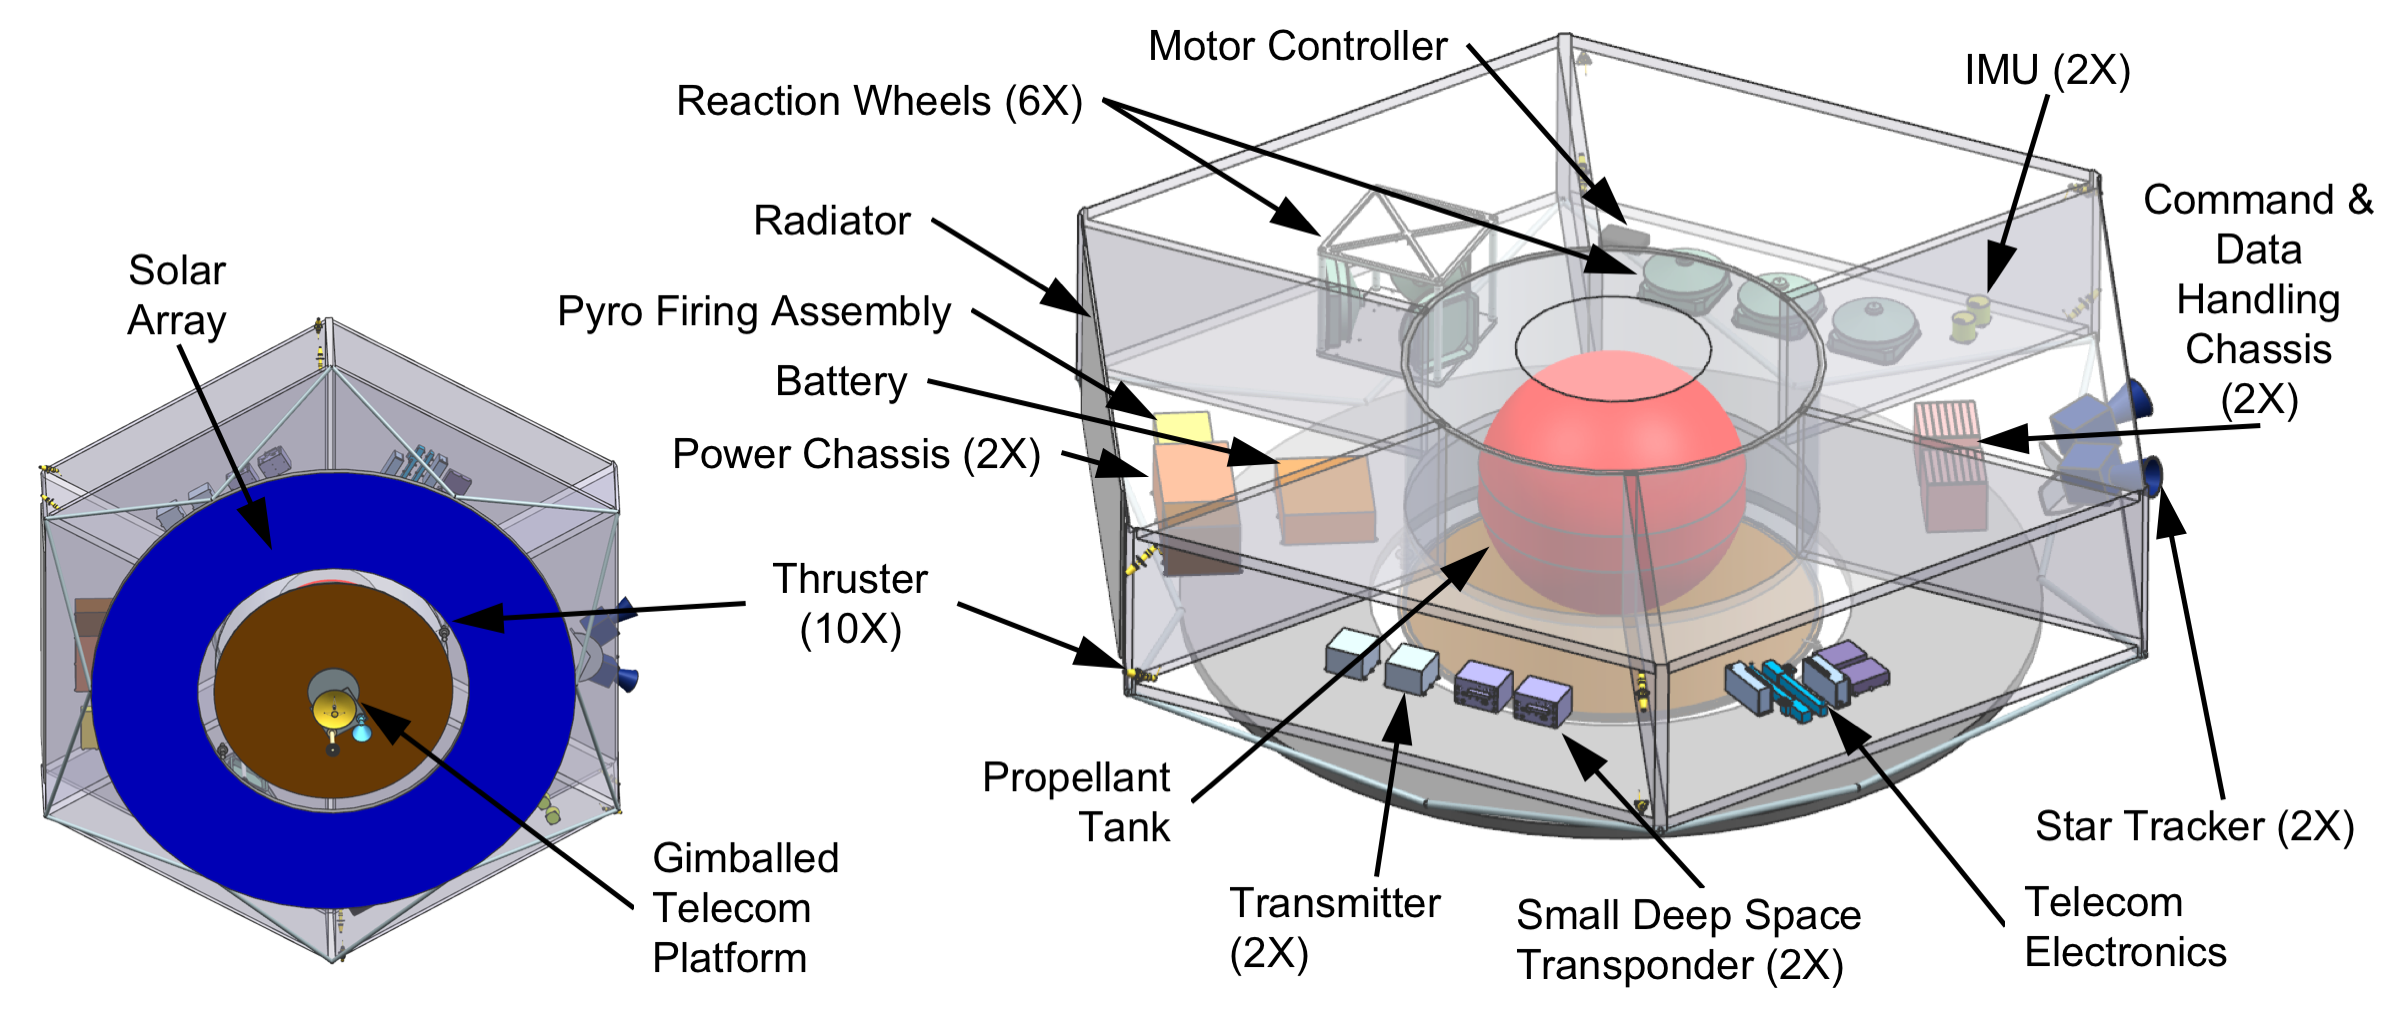
\includegraphics[width=\textwidth]{figures/Spacecraft.png}
\caption{Modular equipment bays provide easy access to all components
  in the spacecraft de-spun module and enable parallel integration of
  spacecraft subsystems.\label{fig:Spacecraft}}
\end{center}
\end{figure}

\subsection{Spacecraft}
\label{sec:spacecraft} %4.3

The PICO spacecraft bus is Class~B and designed for a minimum lifetime of 5\,years in the L2
environment. Mission critical elements are redundant. Flight spares,
engineering models and prototypes appropriate to Class~B are budgeted.

The aft end of the spacecraft (the ``de-spun module'') is comprised of
six equipment bays that house standard components
(Fig.~\ref{fig:Spacecraft}).  The instrument and V-grooves are mounted on
bipods from the spacecraft ``spun module,'' which contains hosted
instrument elements (Fig.~\ref{fig:InstrumentCAD}). A motor drives the
spun module at 1\,rpm to support the science survey requirements
(\S\,\ref{sec:survey_design}). Reaction wheels on the despun module
cancel the angular momentum of the spun module and provide three-axis
control (\S\,\ref{sec:attitude_determination}).

The bipods that mechanically support the instrument are thermally
insulating. The passively radiating V-groove assembly thermally
isolates the instrument from solar radiation and from the bus
(\S\,\ref{sec:radiative_cooling}). Like \textit{Planck} \citep{Tauber2010}, the V-grooves are
manufactured using honeycomb material. Additional radiators on the
spun and despun spacecraft modules ($\sim1$\,m$^2$ each) reject heat
dissipated by spacecraft subsystems and hosted instrument elements.

PICO's avionics are dual-string with standard interfaces. Solid state
recorders provide three days of science data storage (4.6 Tbit), enabling
retransmission of missed data.

PICO employs a fully redundant Ka- and X-band telecommunications
architecture. The Ka-band system uses a 0.3\,m high-gain antenna to
support a science data downlink information rate of 130 Mb/s to a
34\,m BWG DSN ground station with a link margin of 4.8\,dB. The X-band
system provides command and engineering telemetry communication
through all mission phases using medium and low gain
antennas. Amplifiers, switches, and all three antennas are on a
gimballed platform, enabling Ka and X-band downlink concurrent with
science observations.

A 74\,A-hr Li-ion battery is sized for a 3\,hr launch phase with 44\,\% depth of discharge. 
Solar cells on the aft side of the bus provide positive power (with
contingency) for all mission power modes after the launch phase (5.8\,m$^2$ array, $\alpha=26\degree$ off-Sun). The driving
mode is telecom concurrent with science survey (1320\,W including 43\,\% contingency). Unused area in the
solar array plane affords significant margin for growth
(Fig.~\ref{fig:Spacecraft}). The heritage power electronics are dual-string.

The propulsion design is a simple mono-propellant blow-down hydrazine
system with standard redundancy. Two aft-pointed 22\,N thrusters
provide $\Delta V$ and attitude control for orbit insertion and
maintenance (\S\,\ref{sec:mission_design}), requiring 140 kg of
propellant.  Eight 4\,N thrusters provide reaction wheel momentum
management and backup attitude control authority (60\,kg of
propellant). Accounting for ullage (14\,kg), the baseline propellant
tank fill fraction is 77\,\%.


\subsubsection{Attitude determination and control}
\label{sec:attitude_determination} %4.3.1

PICO uses a zero net angular momentum control architecture with
heritage from the SMAP mission (\S\,\ref{sec:heritage}). PICO's instrument
spin rate (1\,rpm) matches that of the \textit{Planck} mission, but
the precession of the spin axis is much faster (10\,hr vs 6\, months),
and the precession angle much larger ($26\degree$ vs
$7.5\degree$). These differences make the spin-stabilized
\textit{Planck} control architecture impractical because of the amount
of torque required to drive precession.

The PICO 1\,rpm instrument spin rate is achieved and maintained using
a spin motor. The spin motor drive electronics provide the coarse spin
rate knowledge used for controlling the spin rate to meet the
$\pm0.1$\,rpm requirement.

Three reaction wheel assemblies (RWAs) are mounted parallel to the
instrument spin axis and spin opposite to the instrument to achieve
zero net angular momentum and keep the despun module three-axis
stabilized. The spin axis is precessed using three RWAs mounted normal
to the spin axis in a triangle configuration. Each set of three RWAs
is sized such that two could perform the required function, providing
single fault tolerance.

Spin axis pointing and spin rate knowledge are achieved and maintained
using star tracker and inertial measurement unit (IMU) data. The
attitude determination system is single-fault tolerant, with two IMUs
each on the spun and despun modules, and two star trackers each on the
spun and despun modules. Two sun sensors on the despun module are used
for safe-mode contingencies and instrument Sun avoidance. All attitude
control and reconstruction requirements are met, including spin axis
control $< 60$\,arcmin with $< 1$\,arcmin/min stability, and
reconstructed pointing knowledge $< 10$\,arcsec (each axis, $3\sigma$).

\newpage
\section{Technology maturation}
\label{sec:technology_maturation} %5

PICO builds off of the heritage of the \textit{Planck} HFI
instrument. Since \textit{Planck}, suborbital experiments have used
monolithically fabricated TES bolometers and multiplexing schemes to
field instruments with thousands of detectors per camera
(Fig.~\ref{fig:spt_fp}).

\begin{figure}
\parbox{3.5in}{\centering
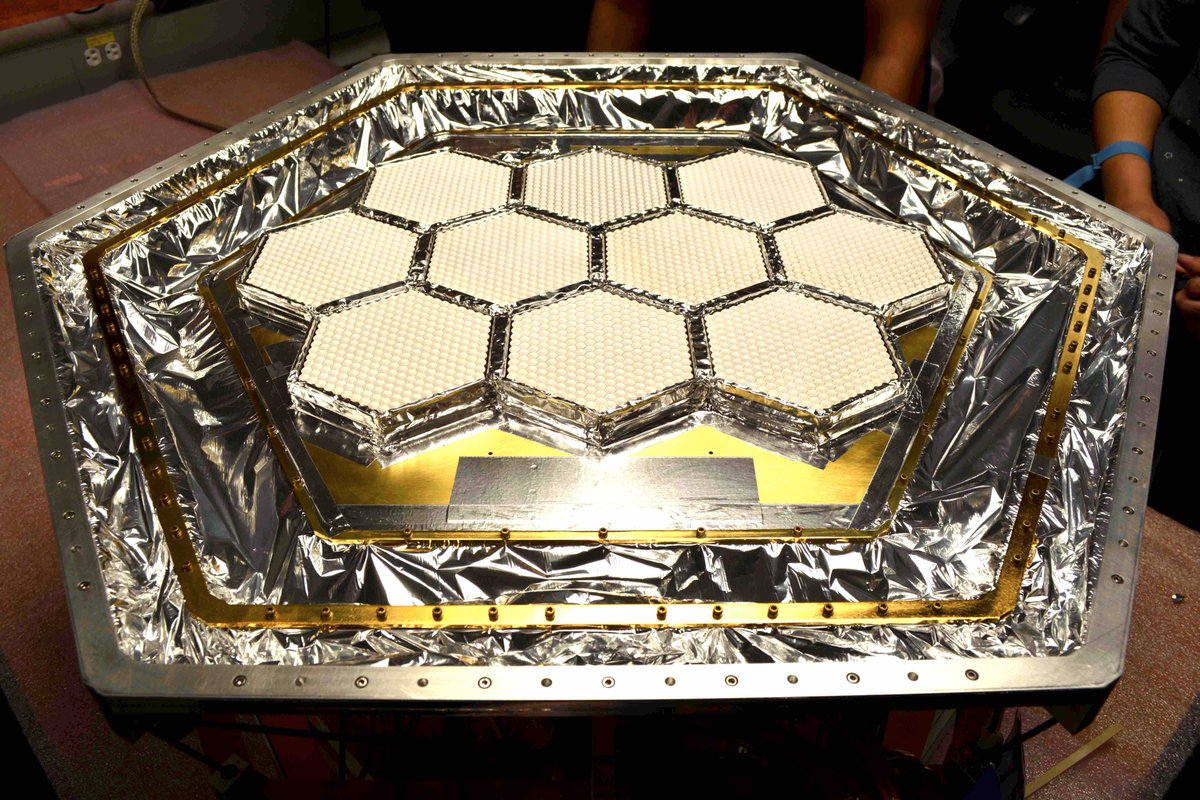
\includegraphics[width=3in]{figures/SPT3G.jpg} }
\parbox{3.0in}{
\caption{SPT-3G operates a focal plane of three-color antenna-coupled pixels with $>16,000$ total bolometers.\label{fig:spt_fp}} }
\end{figure}

 The remaining technology developments required to enable the PICO baseline design are:
\begin{enumerate}
\item Extension of three-color antenna-coupled bolometers down to 21\,GHz and up to 462\,GHz (\S\,\ref{sec:bolometers}).
\item Construction of high-frequency direct absorbing arrays and laboratory testing (\S\,\ref{sec:dev_arrays}).
\item Beam line and 100\,mK testing to simulate the cosmic ray environment at L2 (\S\,\ref{sec:env_testing}).
\item Expansion of time-division multiplexing to support 128 switched rows per readout column (\S\,\ref{sec:multiplexing}).
\item Simulation software (\S\,\ref{sec:simulation}). {\color{red}Shaul to fill this in.}
\end{enumerate}
We recommend APRA and SAT support to complete development of these
technologies through the milestones described in Table~\ref{tab:technologies}.

\begin{table}
\begin{center}
\caption{PICO technologies can be developed to TRL~5 prior to a 2023 Phase~A start using the APRA and SAT programs.\label{tab:technologies}}
%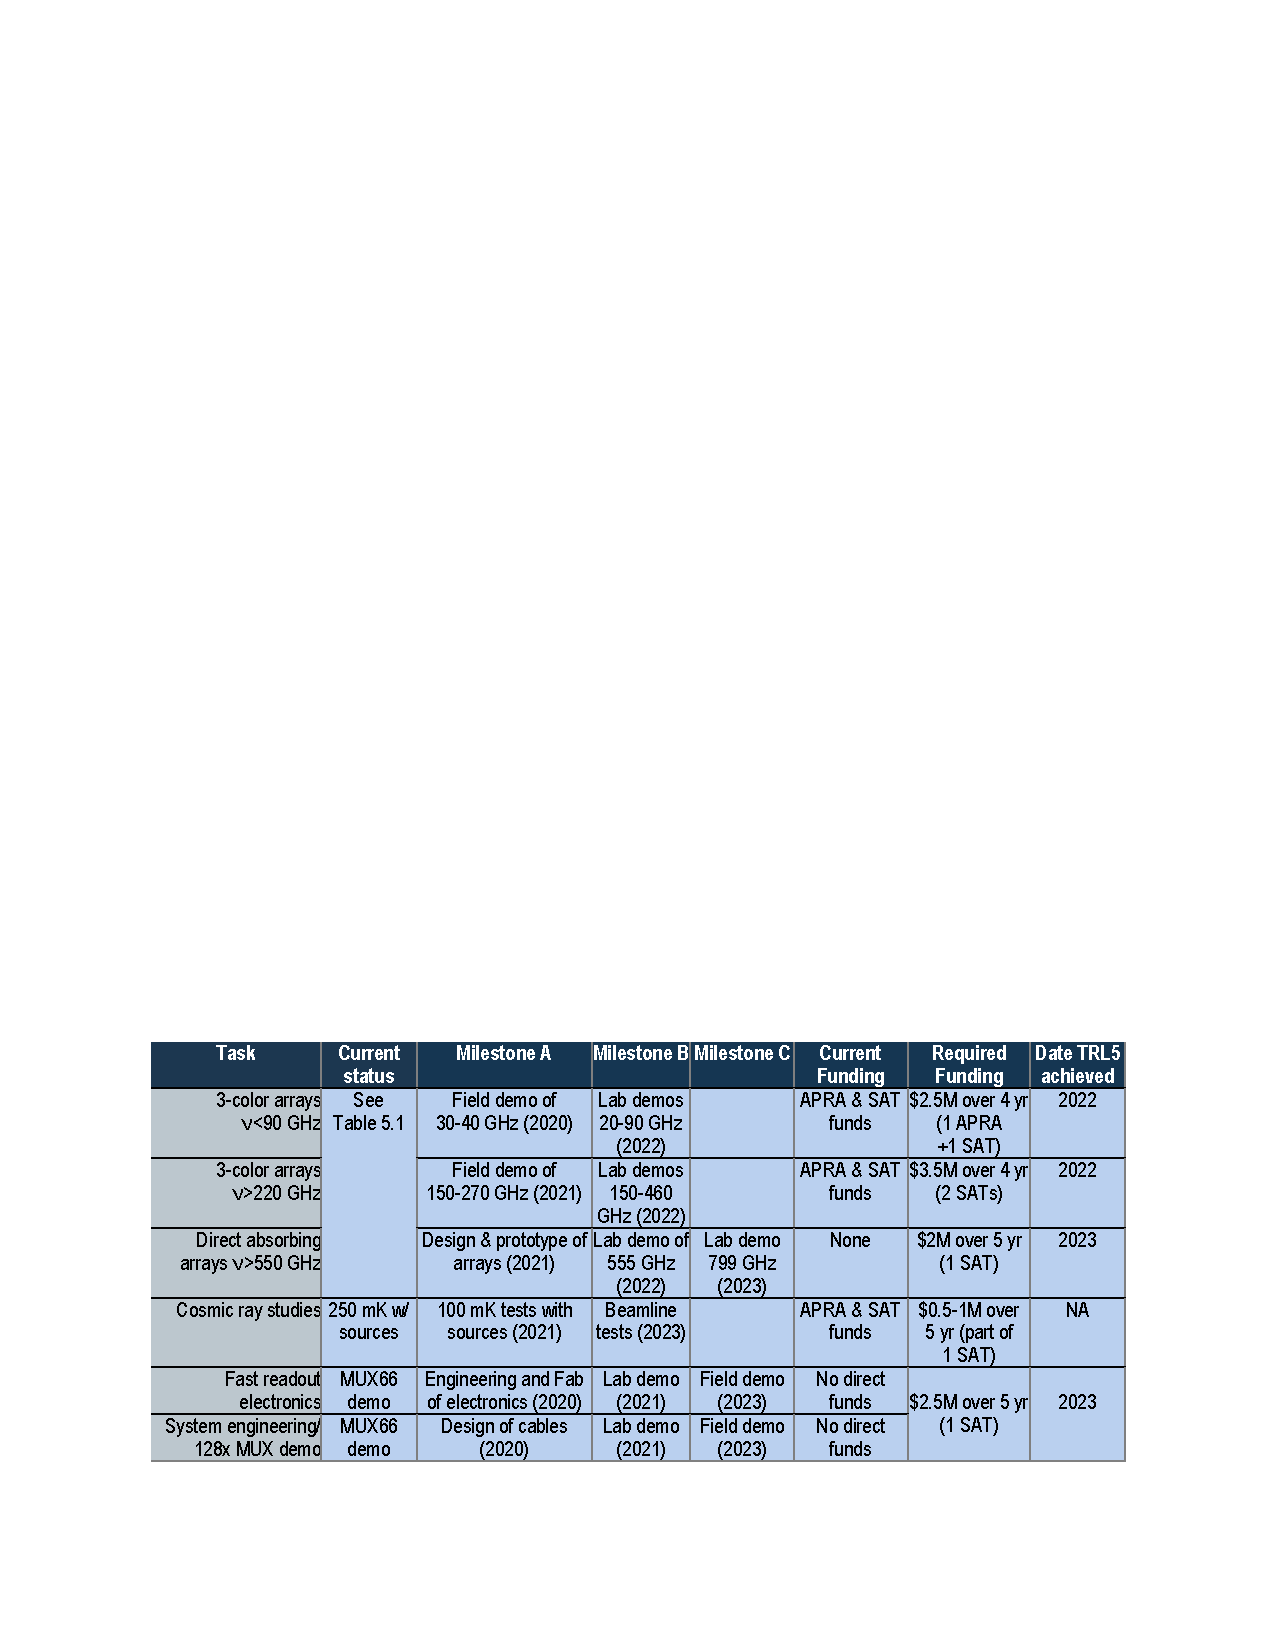
\includegraphics{tables/tab_technologies.pdf}
\begingroup
\setlength{\tabcolsep}{0.5em} 
\renewcommand{\arraystretch}{1.3} % Default value: 1
\scriptsize\rmfamily
\begin{tabular}{lp{1.0in}p{0.75in}p{0.75in}p{0.6in}p{0.6in}p{0.5in}p{0.5in}p{0.4in}}
\hline\noalign{\vskip3pt}
&\bfseries Task & \bfseries Current status & \bfseries Milestone A &\bfseries Milestone B &\bfseries Milestone C &\bfseries Current funding &\bfseries Required Funding & \bfseries TRL5 achieved \\ 
\noalign{\vskip3pt}\hline\noalign{\vskip3pt}
1a.&\parbox[t]{\columnwidth}{Three-color arrays\\$\nu<90$\,GHz} & 2-color lab demos $\nu > 30$\,GHz & Field demo of 30--40\,GHz (2020) & Lab demos 20--90 GHz (2022) & -- & APRA \& SAT funds & \$2.5M over 4\,yr (1 APRA + 1 SAT) & 2022 \\ %\hline
1b&\parbox[t]{\columnwidth}{Three-color arrays\\$\nu > 220$\,GHz} & 2-color lab demos $\nu < 300$\,GHz& Field demo of 150--270\,GHz (2021) &  & -- & APRA \& SAT funds & \$3.5M over 4\,yr (2 SATs) & 2022 \\ %\hline
2.&\parbox[t]{\columnwidth}{Direct absorbing\\arrays $\nu > 50$\,GHz}& 0.1--5\,THz unpolarized&Design \& prototype of arrays (2021)&Lab demo of 555\,GHz (2022)& Lab demo 799\,GHz (2023) & None & \$2M over 5\,yr (1 SAT) & 2023 \\ %\hline
3.&\parbox[t]{\columnwidth}{Cosmic ray studies}& 250\,mK w/ sources&100\,mK tests with sources (2021)&Beamline tests (2023)& -- & APRA \& SAT funds & \$0.5--1M over 5\,yr (part of 1 SAT) & NA \\ %\hline
4a.&\parbox[t]{\columnwidth}{Fast readout\\electronics}& MUX66 demo&Engineering and Fab of electronics (2020)&Lab demo (2021)&Field demo (2023)& No direct funds & \multirow{2}{*}{\parbox[c]{\columnwidth}{\vskip 2.5em\$2.5M over\\ 5\,yr (1 SAT)}} & \multirow{2}{*}{\parbox[c]{\columnwidth}{\vskip 3em 2023}} \\ %\cline{1-7}
4b.&\parbox[t]{\columnwidth}{System engineering;\\ 128x MUX demo} & MUX66 demo &Design of cables (2020)&Lab demo (2021)& Field demo (2023) & No direct funds &  &  \\ %\hline
5.&\parbox[t]{\columnwidth}{Simulation}& &  &  & &  &  & \\
\noalign{\vskip3pt}\hline
\end{tabular}
\endgroup
\end{center}
\end{table}
% ------

% PICO's detector and readout technologies have already been
% substantially matured through complementary suborbital experiments,
% and can be developed by the APRA and SAT programs to NASA's Technology
% Readiness Level (TRL)~5 before Phase~A (October 2023) (Table~\ref{tab:technologies}).
% % The 4\,K cryocooler baselined by PICO requires only standard thermal engineering (\S\,\ref{sec:4kcooler}).

% \subsection{Current state of technologies}
% \label{sec:current_state} %5.1

% PICO builds off of the heritage of the \textit{Planck} HFI
% instrument. Since \textit{Planck},
% numerous suborbital experiments have used monolithically fabricated
% TES bolometers and multiplexing schemes to field instruments with
% thousands of detectors per camera (Table~\ref{tab:suborbital})

\subsection{Three-color antenna-coupled bolometers}
\label{sec:bolometers} %5.1

Suborbital teams have successfully demonstrated a variety of optical
coupling schemes, including horns with ortho-mode transducers (OMTs),
lithographed antenna arrays, and sinuous antennas under lenslets
(Fig.~\ref{fig:OpticalCoupling}). All have achieved
background-limited performance in suborbital instruments with
sufficient margin on design parameters to achieve this performance in
the more demanding low background at L2.  Experiments have covered
many of PICO's observing bands between 27\,GHz and 270\,GHz
(Table~\ref{tab:suborbital}). SPT-3G has used the PICO-baselined
three-color pixel design to deploy 16,260 detectors covering
90--150--220\,GHz. Other experiments have successfully deployed
two-color pixels. All of these detector arrays have been packaged into
modules and focal plane units in working cameras representative of the
PICO integration.

To date, suborbital experiments have achieved statistical map depths
of 3\,$\mu$K$_{\rm CMB}$\,arcmin on degree-scaled modes over small
parts of the sky, within an order of magnitude of what PICO achieves over the entire
sky (Table~\ref{tab:bands}), and have demonstrated systematic control
better than this level through full-pipeline simulations and null-test analysis
(jackknife tests). 

The baseline PICO instrument requires three-color dual-polarized
antenna-coupled bolometers covering bands from 21 to 462\,GHz and
single-color dual-polarized direct-absorbing bolometers from 555 to
799\,GHz (\S\,\ref{sec:low_freq_det}.
The extension to lower frequencies requires larger antennas and
therefore control of film properties and lithography over larger
areas. Scaling to higher frequencies forces tighter critical
dimensions and materials tend to exhibit higher losses. These
challenges require tight control of cleanliness and full understanding
of process parameters. All developments require careful
characterization of beam properties and studies of associated
systematic challenges for PICO.

The sinuous antenna has the bandwidth to service three colors per
pixel, whereas horns and antenna arrays have only been used for two,
so some version of the sinuous antenna will likely be needed to
realize three-color pixels. However, the sinuous antenna couples to
states that ``wobble'' log-periodically with frequency. There are
potential solutions to this in the focal plane design, analysis, and
free parameters of the antenna geometry. These will need to be
explored subject to the uniformity and packing density constraints
present at the extreme spectral bands.  Systematics studies for field
demonstrations will be particularly important. The PICO concept is
robust to any challenges in developing three-color pixels;
\S\,\ref{sec:technology_descopes} describes an option to descope to
two-color pixels.

\begin{figure}
  \begin{minipage}[b]{0.475\textwidth}
    \begin{center}
    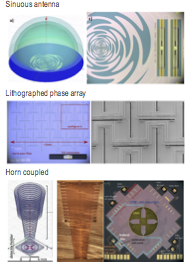
\includegraphics[width=2.5in]{figures/OpticalCoupling.png}
    \caption{Multiple demonstrated optical coupling schemes are available   to PICO. Images from CMB-S4 Technology Book   \citep{Abitbol2017}.\label{fig:OpticalCoupling}}
   \end{center}
  \end{minipage}
  %
  \hfill
  \begin{minipage}[b]{0.475\textwidth}
    \begin{center}
    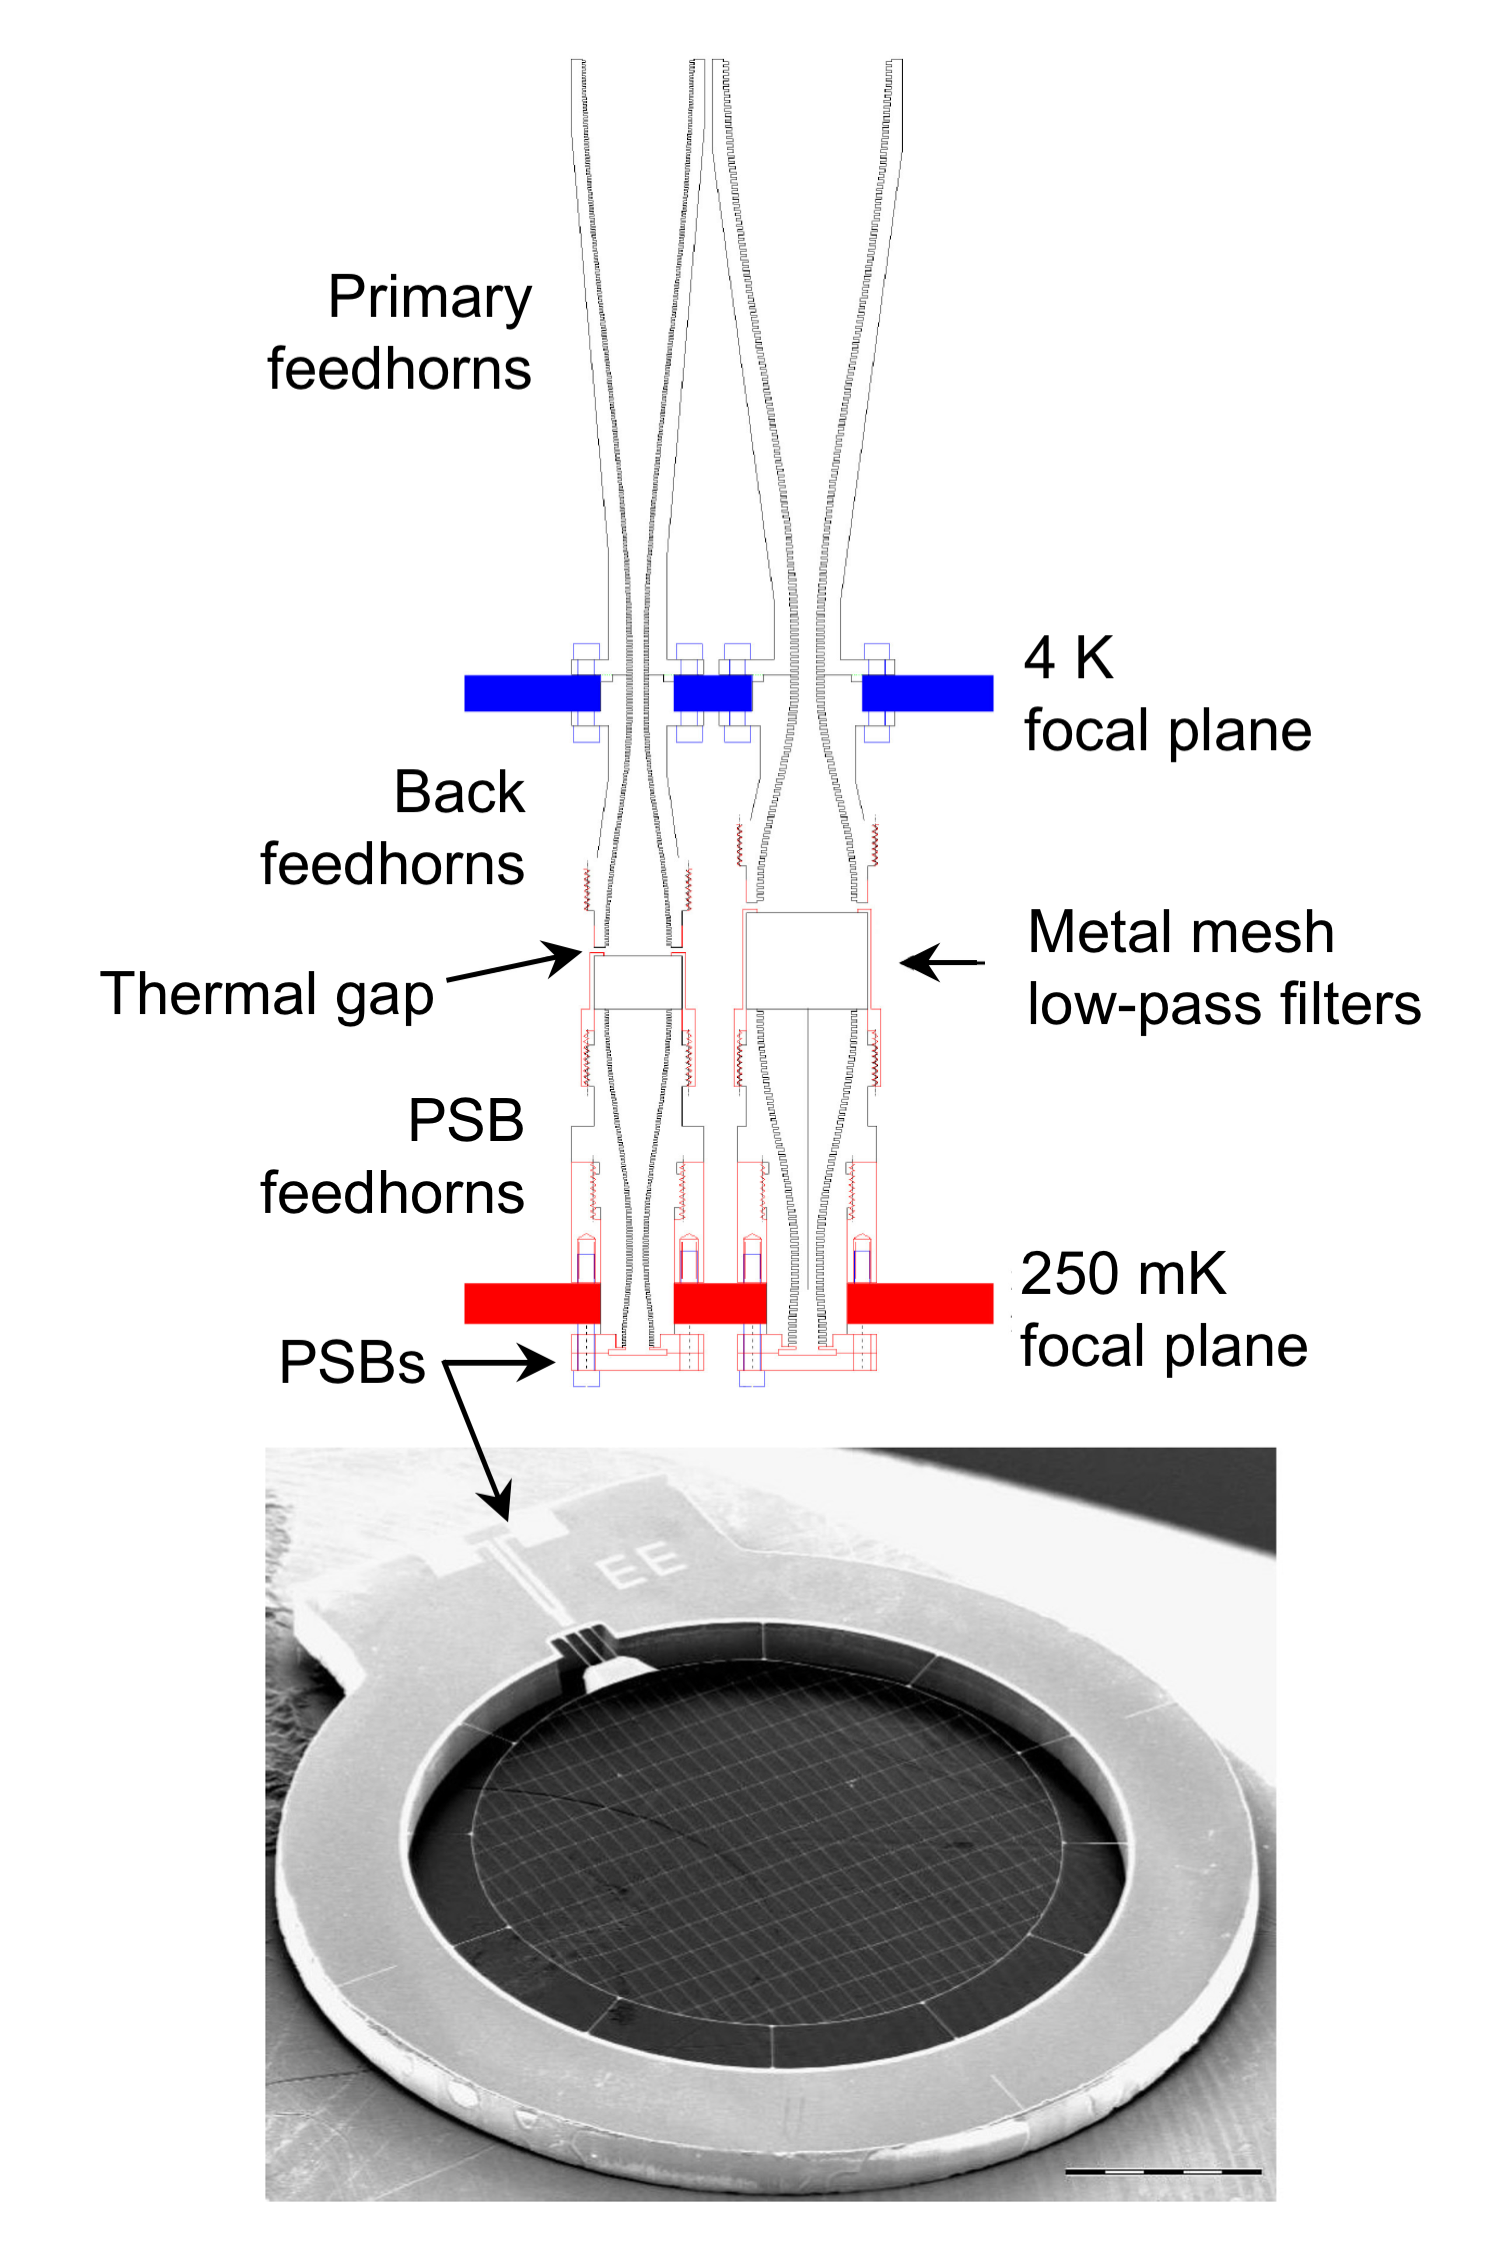
\includegraphics[width=2.5in]{figures/DirectAbsorbing.png}
    \caption{Direct-absorbing dual-polarized detectors and coupling horns used in \textit{Planck} for 143--343\,GHz bands.\label{fig:DirectAbsorbing}}
    \end{center}
  \end{minipage}
\end{figure}

% \begin{figure}
% \begin{center}
% 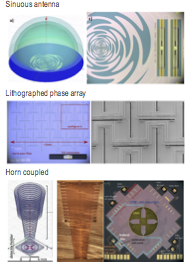
\includegraphics[width=3in]{figures/OpticalCoupling.png}
% \caption{Multiple demonstrated optical coupling schemes are available
%   to PICO. Images from CMB-S4 Technology Book
%   \citep{Abitbol2017}.\label{fig:OpticalCoupling}}
% \end{center}
% \end{figure}

% \begin{figure}
% \begin{center}
% 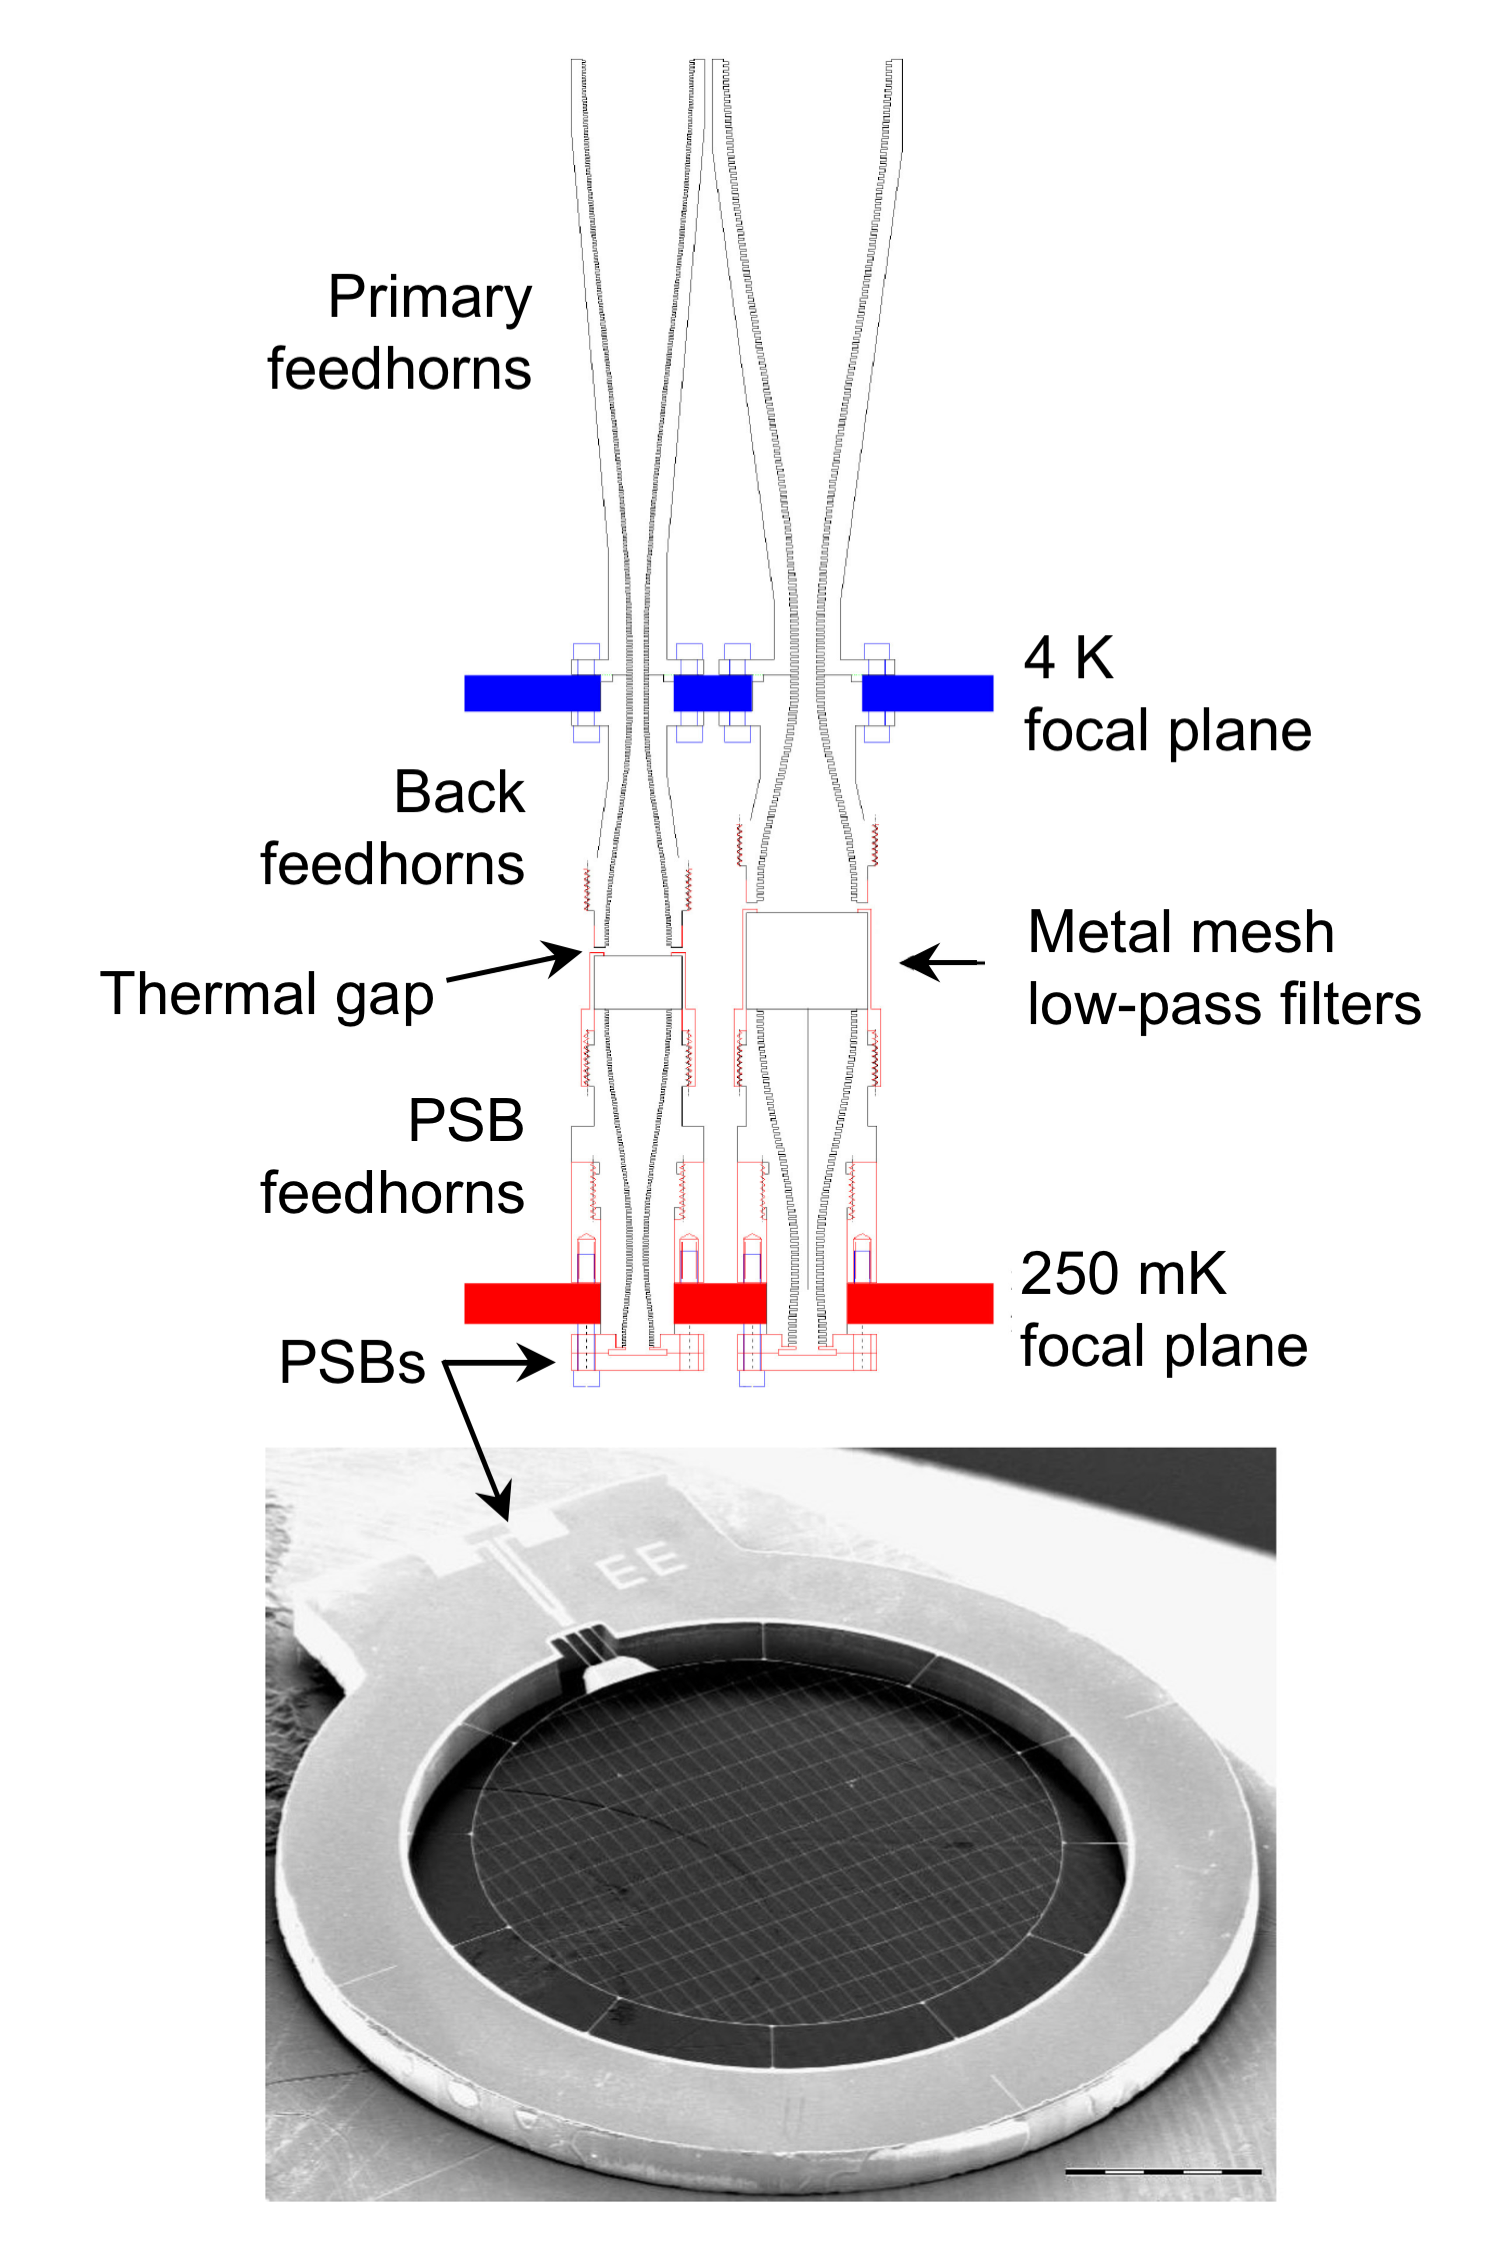
\includegraphics[width=3in]{figures/DirectAbsorbing.png}
% \caption{Direct-absorbing dual-polarized detectors and coupling horns used in \textit{Planck} for 143--343\,GHz bands.\label{fig:DirectAbsorbing}}
% \end{center}
% \end{figure}

\subsection{High-frequency direct absorbing arrays}
\label{sec:dev_arrays}

The baseline PICO instrument requires single-color dual-polarized
direct-absorbing bolometers from 555 to 799\,GHz (\S\,\ref{sec:high_freq_det}).

Ground and balloon experiments have deployed focal planes with
hundreds of horn-coupled spiderweb bolometers. SPT-Pol deployed
dual-polarized versions of direct absorber horn-coupled
bolometers. \textit{Planck} used this style of bolometer, but with NTD-Ge
thermistors instead of TESs (Fig.~\ref{fig:DirectAbsorbing}). Filled arrays of detectors
such as Backshort Under Ground (BUG) bolometers are also an option for
these channels. The status of these efforts is summarized in Table~\ref{tab:technologies}.

\textit{Planck} demonstrated the architecture of horns coupled to direct
absorbing bolometers. For PICO's high frequency detectors, this only
needs to be generalized to dual polarized arrays. The greatest
remaining challenge is the low-risk development of a packaging
design. Such prototyping could culminate in a field demonstration,
best performed in a balloon.

\subsection{Environmental testing}
\label{sec:env_testing}
Laboratory tests and in-flight data from
balloons suggest that these TES bolometers are more naturally robust
against cosmic rays than the individual NTD-Ge bolometers used in
\textit{Planck}. Cosmic ray glitches have fast recovery times and low
coincidence rates \citep{SPIDER2018}.

So far, cosmic ray tests and in-flight analysis of TES bolometers are
encouraging \citep{SPIDER2018}. The CMB community can retire residual
risk with 100\,mK testing where the array heat sinking may be weaker,
and beam-line tests to help control for background glitch rates.

\subsection{Multiplexing}
\label{sec:multiplexing}

More than ten experiments have used TDM readout. SCUBA2 on JCMT has
10,000 pixels, nearly as many detectors as planned for PICO
\citep{Holland2013}. Most of these experiments have used 32-row
multiplexing. Recently ACT has expanded this to 64-row multiplexing \citep{Henderson2016}.

PICO's sensitivity requirements dictate the use of $\sim 13,000$
transition edge sensor bolometers, requiring a highly multiplexed
system.  The PICO baseline design calls for time-division multiplexing
with 128 switched rows per readout column (TDM-128$\times$), which
exceeds that of Advanced ACTPol's recently demonstrated TDM-66$\times$
\citep{Henderson2016}. The leap to TDM-128$\times$ requires:
\begin{itemize}
\item development of fast-switched room temperature electronics; and
\item system engineering of room temperature to cryogenic row select cabling to ensure sufficiently fast row switch settling times.
\end{itemize}
The system engineering study should culminate in a demonstration of TDM-128$\times$ SQUID aliased noise below PICO detector sensitivity requirements.  

\subsection{Simulation}
\label{sec:simulation}

{\color{red} Shaul to write/delegate this section.}

% \subsubsection{Readout electronics status}
% \label{sec:readout_status} %5.1.2



\begin{table}
\begin{center}
\caption{Multiple active suborbital efforts are advancing technologies relevant to PICO.\label{tab:suborbital}}
%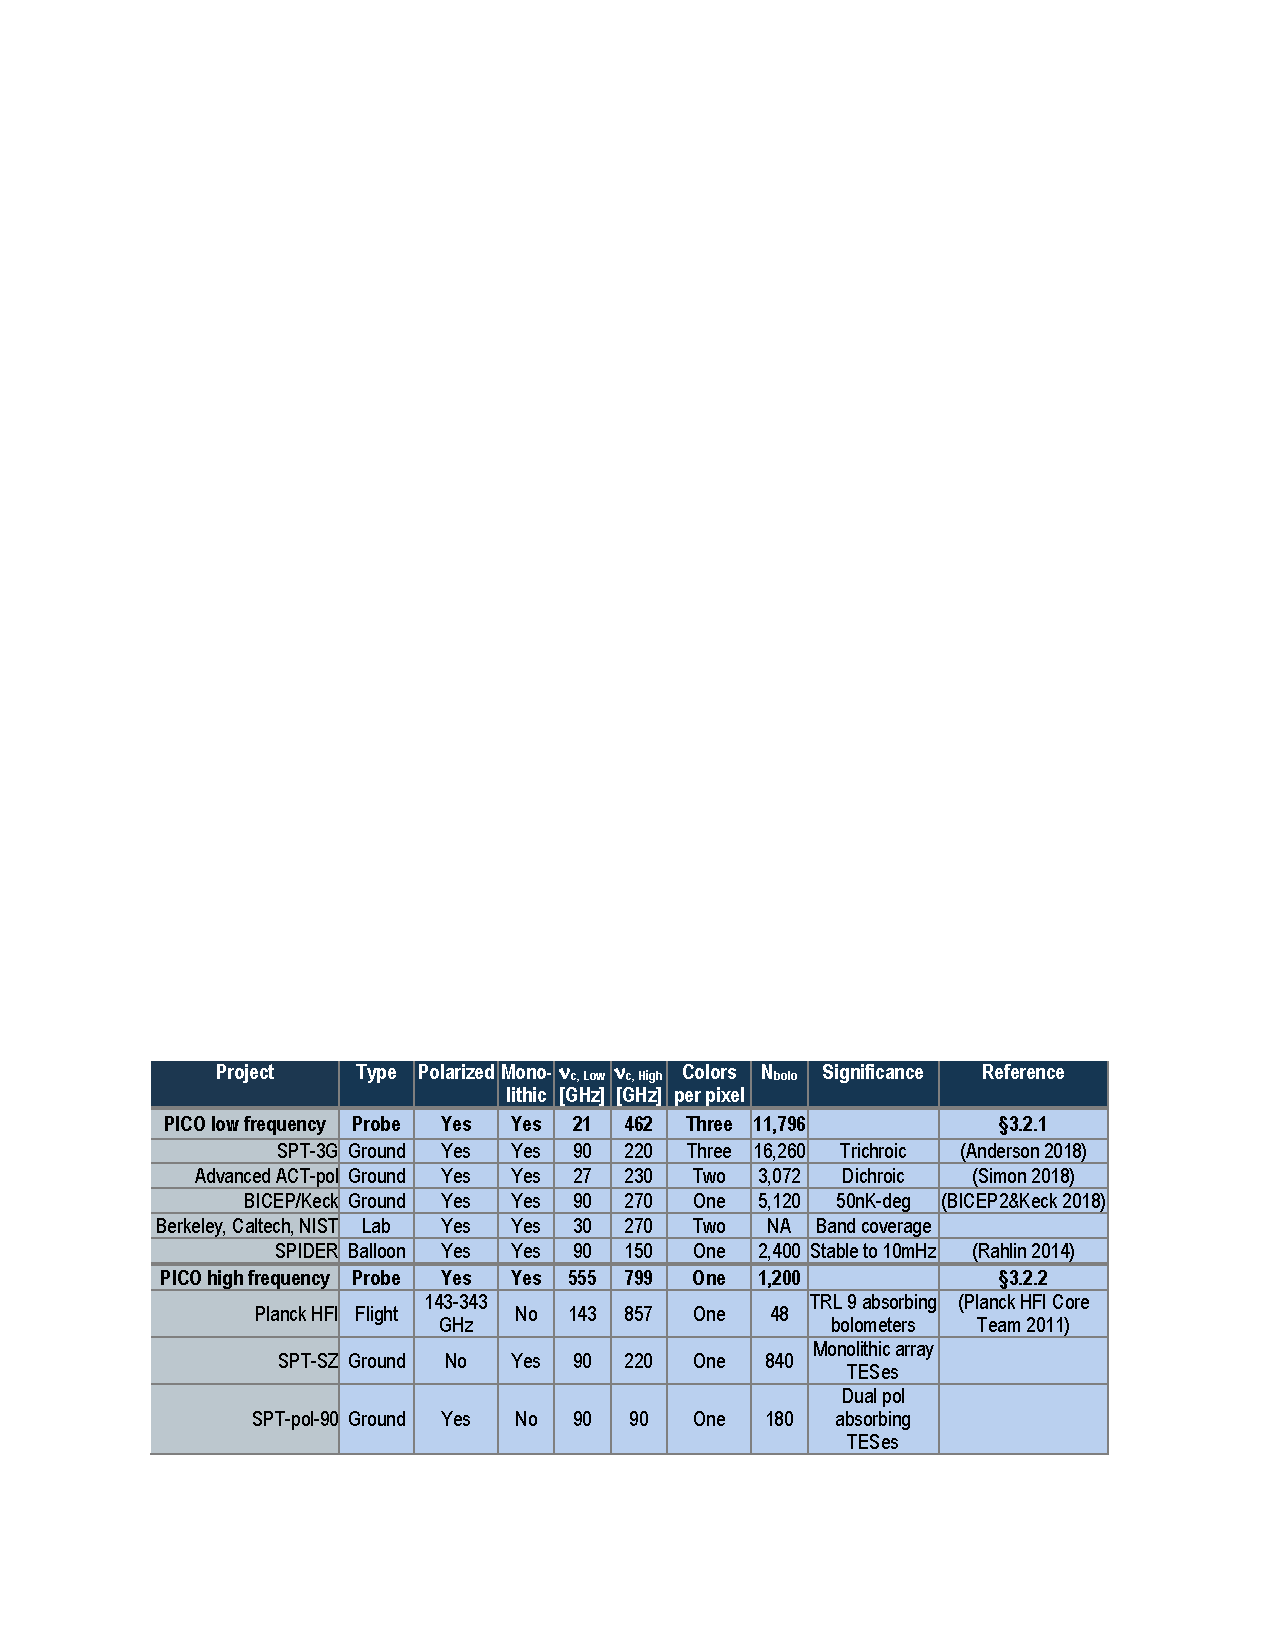
\includegraphics{tables/tab_suborbital.pdf}
\scriptsize\rmfamily
\begin{tabular}{lccccccp{0.75in}c}
\hline\noalign{\vskip3pt}
Project&Type&Polarized&Mono-&$\nu_c$&Colors&$N_{\rm bolo}$&Significance&Reference\\
           &       &              &lithic?  &[GHz]&per pixel&\\
\noalign{\vskip3pt}\hline\noalign{\vskip3pt}
PICO low frequency&Probe&Yes&Yes&21 -- 462&Three&11,796&&\S\,\ref{sec:low_freq_det}\\
SPT-3G&Ground&Yes&Yes&90 -- 220&Three&16,260&Trichroic&\cite{Dutcher2018}\\
Advanced ACT-pol&Ground&Yes&Yes&27 -- 230&Two&3,072&Dichroic&\cite{Li2018}\\
BICEP/Keck&Ground&Yes&Yes&90 -- 270&One&5,120&50\,nK-deg&\cite{bicep_keck2018}\\
Berkeley, Caltech, NIST&Lab&Yes&Yes&30 -- 270&Two&--&Band coverage&\cite{Westbrook2016,Hui2018,Simon2018}\\
SPIDER&Balloon&Yes&Yes&90 -- 150&One&2,400&Stable to 10\,mHz&\cite{Rahlin2014}\\
\noalign{\vskip3pt}\hline\noalign{\vskip3pt}
PICO high frequency&Probe&Yes&Yes&555 -- 799&One&1,200&&\S\,\ref{sec:high_freq_det}\\
Planck HFI&Flight&Yes*&No&143 -- 857&One&48&TRL 9 absorbing bolometers&\cite{Turner2001}\\
SPT-SZ&Ground&No&Yes&90 -- 220&One&840&Monolithic array TESs&\cite{Shirokoff2011}\\
SPT-pol-90&Ground&Yes&No&90&One&180&Dual pol absorbing TESs&\cite{Sayre2012}\\
\noalign{\vskip3pt}\hline
\end{tabular}
\vskip5pt {\scriptsize * 143--343\,GHz only}
\end{center}
\end{table}

% \subsection{Development plan}
% \label{sec:development_plan}  %5.2

% \subsubsection{Detector development}
% \label{sec:detector_development} %5.2.1

% .

% \textit{Planck} demonstrated the architecture of horns coupled to
% direct absorbing bolometers. For PICO's high frequency detectors, this
% only needs to be generalized to dual polarized arrays. The greatest
% remaining challenge is the low risk development of a packaging
% design. Such prototyping could culminate in a field demonstration,
% best performed in a balloon.


% A plan to accomplish all required development is described in rows 1--4 of Table~\ref{tab:technologies}.


% \subsubsection{Readout electronics development}
% \label{sec:readout_development} %5.2.2


% A plan to accomplish the required development is described in rows 5 and 6 of Table~\ref{tab:technologies}.

\subsection{Technology descopes}
\label{sec:technology_descopes} %5.3

A descope from three-color to two-color pixels remains a viable
alternative should the three-color technology not mature as
planned. Descope studies suggest that a PICO-size focal plane using
two-color pixels at the lower frequencies and the baseline one-color
pixels at the higher frequencies would contain 8,840 detectors
(compared to the baseline 12,966) and map in 19 colors (baseline
21). Because horns have a $2.3:1$ bandwidth, each of the two bands in
a pixel has 35\,\% bandwidth (compared to the baseline 25\,\%), which
compensates for pixel count, resulting in
0.61\,$\mu$K$_{\rm CMB}$\,arcmin aggregate CBE map depth, which
matches the PICO CBE map depth, and affords $>40\,\%$ margin against
the 0.87\,$\mu$K$_{\rm CMB}$\,arcmin baseline requirement
(Table~\ref{tab:bands}), but with coarser spectral resolution.

\subsection{Enhancing technologies}
\label{sec:enhancing_technologies} %5.4

The following technologies are neither required nor assumed by the
PICO baseline concept. They represent opportunities to extend
scientific capabilities or simplify engineering.

PICO baselines TDM readout because of its relative maturity and
demonstrated sensitivity and stability in relevant science
missions. Lab tests of Frequency Domain Multiplexing (FDM) suggest
comparable performance with higher multiplexing factors and lower
loads on cryogenic stages relative to TDM. Suborbital experiments such
as SPT-3G have used frequency division multiplexing (FDM) to readout
focal planes comparable in size to PICO.

Microwave frequency SQUID multiplexing can increase the multiplexing
density and reduce the number of lines between the 4K and ambient
temperature stages \citep{Dober2017,Irwin2004}. Kinetic Inductance
Detectors (KIDs) and Thermal KIDs (TKIDs) can further reduce the wire
count, obviate the SQUIDs, and dramatically simplify integration by
performing multiplexing on the same substrate as the detectors
themselves \citep{McCarrick2016,Steinbach2018}. The cost to develop
these technologies is \$3--4M/year, with a high chance of reaching
TRL-5 before Phase~A.

\newpage
\section{Project management, heritage, risk, and cost}
\label{sec:project_management} %6

\subsection{PICO Study Participants}
\label{sec:study_participants} %6.1

The PICO study was open to the entire mm/sub-mm science community and
included more than 150 scientists. Seven working groups were led by
members of PICO's Executive Committee, which met weekly under the
leadership of PI Shaul Hanany. More than 60 people participated
in-person in two community workshops (November 2017 and May 2018).

The PICO engineering concept definition package was generated by
Team~X (the JPL concurrent design lab). The Team X study was supported
by inputs from a JPL engineering team and Lockheed Martin.

The full list of study report contributors and endorsers follows the cover page.

\subsection{Project management plan}
\label{sec:management_plan} %6.2

PICO benefits from the experience of predecessor missions such as
\textit{Planck} and \textit{WMAP}, as well as many years of investment
in technology development and a multitude of suborbital
experiments. In addition to demonstrated science and engineering
capabilities, this heritage has developed a community of people with
the expertise required to field a successful mission.

This study assumes mission management by JPL with a Principal
Investigator leading a single science team. A Project Manager provides
project oversight for schedule, budget, and deliverables. A Project
Systems Engineer leads systems engineering activities and serves as
the Engineering Technical Authority. A Mission Assurance Manager
serves as the Independent Technical Authority. The PICO mission
development schedule is shown in Fig.~\ref{fig:Schedule}.

\begin{figure}[hb]
\begin{center}
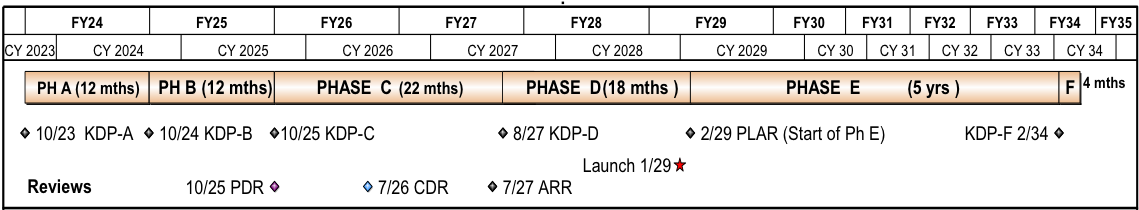
\includegraphics[width=\textwidth]{figures/Schedule.png}
\caption{The PICO baseline schedule is based on historical actuals
  from similarly-sized missions such as Juno and
  SMAP. Per NASA direction, Probe studies assume a Phase~A start in October 2023.\label{fig:Schedule}}
\end{center}
\end{figure}

Probes are medium-class missions, similar in cost scope to NASA's
New Frontiers missions, which are Category~1 and Risk Classification A
or B, with Phase A--D costs capped at $\sim$ \$850M (not including the
launch vehicle). JPL is well-prepared to manage Probe missions, having
managed the Juno New Frontiers mission (launched 2011) and also the
development of the medium-class \textit{Spitzer} Space Telescope (launched
2003). JPL delivered the bolometric detectors for the \textit{Planck}
HFI instrument (launched 2009). Presently, JPL is managing NEOCam, a
Discovery class infrared space telescope.

The PICO spacecraft provider will be selected during mission
formulation. Multiple organizations are capable of providing a
spacecraft bus to meet PICO's requirements. Lockheed Martin
contributed to the PICO concept study, leveraging their experience
with New Frontiers missions Juno and OSIRIS-REx.
 
\subsection{Heritage}
\label{sec:heritage} %6.3

The successful \textit{Planck} mission provides science heritage for
PICO. Technical heritage traces to multiple missions.

Because PICO observes in the mm/sub-mm regime, the surface accuracy
requirement for the reflectors is relatively easy to meet. PICO's
reflectors are similar to \textit{Planck}'s, but somewhat larger
($270\,{\rm cm} \times 205\,{\rm cm}$ primary vs.\
$189\,{\rm cm} \times 155\,{\rm cm}$)
\citep{Gloesener2006}. \textit{Herschel} observed at wavelengths more
demanding than PICO's and was larger ($350\,{\rm cm}$ diameter
primary) \citep{Toulemont2004}.

The heritage of the PICO detectors and readout electronics
(\S\,\ref{sec:focal_plane}, \S\,\ref{sec:detector_readout}) is
described in \S\,\ref{sec:technology_maturation}.


PICO's detectors are cooled by a cADR (\ref{sec:cadr}) with
requirements that are within the capabilities of current ADRs
developed by Goddard Space Flight Center. These systems have been
applied to several JAXA missions, including \textit{Hitomi} \citep{Shirron2016}.

PICO's 4\,K cryocooler (\S\,\ref{sec:4kcooler}) is a direct extension
of the JWST MIRI design \citep{Durand2008,Rabb2013}. PICO benefits
from a simpler and more reliable implementation of the J-T system than
was required for MIRI, in that no deployment of cooling lines is
required, and all flow valving is performed on the warm
spacecraft. Cooling multiple independent points with a J-T loop has
been demonstrated on \textit{Planck} with the JPL-supplied 18\,K
cooler \citep{Planck2011}.

Structures similar to PICO's V-groove radiator assembly
(\S\,\ref{sec:radiative_cooling}) are a standard approach for passive
cooling first described more than thirty years ago
\citep{Bard1987}. 
%PICO's 4.5\,m diameter V-groove assembly fits inside the launch vehicle fairing. 
PICO
has baselined a simple honeycomb material construction like that
successfully flown by the \textit{Planck} mission
\citep{ESA2009,Planck2011}.

Most requirements on the PICO spacecraft are well within typical
ranges and can be met with standard high heritage systems
(\S\,\ref{sec:spacecraft}). PICO's spin architecture and data volume
requirements are less typical, and discussed below.

The PICO zero-momentum control architecture
(\S\,\ref{sec:attitude_determination}) has heritage from the SMAP
mission's successful control architecture. PICO has a slower spin rate and less cancelled angular
momentum than SMAP. SMAP requires 359\,N\,m\,s to cancel the momentum of a
6\,m instrument antenna spun at 14.6\,rpm \citep{Brown2016}. 
Based on mass properties derived from the PICO CAD model, PICO requires XXX N\,m\,s to cancel the momentum of the instrument and spacecraft spun module (XXX\,kg including contingency) at 1\,rpm. 
%The PICO launch
% mass (2147\,kg including contingency) is similar to the \textit{Planck} launch mass (1912\,kg \citep{Tauber2010}. If
% we assume \textit{Planck} moments of inertia \citep{ESA2016}, the PICO spun elements
% would have an angular momentum of 210\,N\,m\,s at 1\,rpm. This is
% conservative because, unlike \textit{Planck}, the entire PICO
% observatory does not spin.

Though PICO's data volume is notable by current standards, it is
already enveloped by missions in development. PICO produces
6.1\,Tb/day of raw data which is compressed to 1.5\,Tb/day
(\S\,\ref{sec:detector_readout}). PICO downlinks data daily, but
baselines storage of 3\,days of (compressed) data to mitigate missed
telecom passes. This requires 4.5\,Tb of onboard storage, in family
with the 3.14\,Tb solid state recorder currently in use by Landsat~8
and much smaller than the 12\,Tb flash memory planned for NISAR
\citep{Jasper2017}. The PICO baseline 150\,Mb/s Ka-band data downlink
is an existing DSN catalog service \citep{DSN2015}. The
baseline PICO mission generates $\sim2,200$\,Tb of raw (uncompressed)
data per year, less than the $\sim6,800$\,Tb/year currently returned
by Landsat~8 and $\sim 9,300$\,Tb/yr planned by NISAR
\citep{Jasper2017}.

\subsection{Risk assessment}
\label{sec:risk_assessment} %6.4

\subsubsection{Pre-mission risks}
\label{sec:premission_risks} %6.4.1

Technology development (\S\,\ref{sec:technology_maturation}) is
performed prior to the beginning of mission development, and is
outside of the mission cost (per NASA direction), so associated risks
do not represent threats to the cost of mission development. Rather,
these technology development risks affect 
the availability of the described baseline
mission. A technology-related mission descope is described in
\S\,\ref{sec:technology_descopes}.

\subsubsection{Development risks}
\label{sec:development_risks} %6.4.2

PICO's healthy contingencies, margins, and reserves provide
flexibility to address risks realized during mission development. PICO
carries $>40\,\%$ instrument sensitivity margin (Table~\ref{tab:bands}),
$>100\,\%$ heat lift margin (Table~\ref{tab:cooler}), $43\,\%$ system
power contingency, $31\,\%$ payload mass contingency, and $25\,\%$
spacecraft mass contingency. The Falcon~9 launch capability (assuming ocean
recovery) exceeds PICO's total launch mass (including contingency) by
a $\sim 50\,\%$ margin. The PICO budget includes $30\,\%$ cost
reserves for Phases A--D (\S\,\ref{sec:mission_cost}).

During mission development the Project Systems Engineer continually
assesses risks, tracks progress toward retiring them, and updates
mitigations. Mitigations for a few top risks identified during this
study are described below.
\begin{itemize}
\item Thermal risk can be mitigated through extensive thermal modeling and
review in Phase A, and design for early test verification. 
\item Risks
associated with the instrument spin architecture can be mitigated by
engaging JPL engineers who were involved in the SMAP mission.
\item  Detector
delivery schedule risk can be mitigated by beginning fabrication early
in the project life cycle and fabricating a generous number of
detector wafers to ensure adequate yield. Multiple institutions (including, for example, JPL, GSFC, NIST, and ANL) would be capable of producing the PICO detectors. Suborbital programs generally achieve $>66\,\%$ detector wafer yield.
\item Risks associated with the
integration and test of a cryogenic instrument can be mitigated
through advanced planning and allocation of appropriate schedule and
schedule margin.
\end{itemize}

\subsubsection{Operations risks}
\label{sec:operations_risks} %6.4.3

The PICO design meets the requirements associated with the NASA
Class~B risk classification. For Class~B missions, essential
spacecraft and instrument functions are typically fully
redundant. This increases mission cost, but significantly reduces the
risk of mission failure.

The PICO mission utilizes a single instrument with a single observing
mode mapping the sky using a repetitive survey pattern. The mission
does not require any time-critical activities. The observatory fits in
to the launch vehicle fairing in its operational configuration, so no
hardware deployments are required. Because PICO observes at long
wavelengths, the telescope does not require a dust cover (nor the
associated mission-critical cover release).

The spacecraft incorporates a fault protection system for anomaly
detection and resolution. The Sun-pointed, command receptive,
thermally stable safe-mode attitude allows ground intervention for
fault resolution without time constraints. PICO's high degree of
hardware redundancy and onboard fault protection ensure spacecraft
safety in the event of unforeseen failures and faults.

Science data analysis, including foreground separation
(\S\,\ref{sec:signal_separation}) and systematics control (\S\,\ref{sec:systematics}) are
discussed in the science section (\S\,\ref{sec:science}).

\subsection{Mission cost}
\label{sec:mission_cost} %6.5
 
We estimate PICO's total Phase A--E lifecycle cost between \$870M and
\$960M, including the \$150M allocation for the Launch Vehicle (per
NASA direction). These cost estimates include 30\,\% reserves for
development (Phases A--D) and 13\,\% reserves for operations
(Phase~E). Pre-Phase-A technology maturation
(\S\,\ref{sec:technology_maturation}) will be accomplished through the
normal APRA and SAT processes, and is not included in the mission cost
(per NASA direction).

Table~\ref{tab:cost} shows the mission cost breakdown, including the
JPL Team~X cost estimate as well as the PICO team cost estimate. Team~X
 is JPL's concurrent design facility. Team~X estimates are generally
model-based, and were generated after a series of instrument and
mission-level studies. Their accuracy is commensurate with the level
of understanding typical to Pre-Phase-A concept development. They do
not constitute an implementation or cost commitment on the part of JPL
or Caltech.

\begin{table}
\centering
\caption{Detailed breakdown of Team X and PICO Team cost estimates (in FY18\$). Costs are based on the schedule in Fig.~\ref{fig:Schedule}, which includes 5~years of operations.}\label{tab:cost}
\footnotesize\rmfamily
\begin{tabular}{p{2.5in}cc}
\hline\noalign{\vskip3pt}
\textbf{Work Breakdown Structure (WBS) Elements}&\textbf{Team~X}&\textbf{PICO Team}\\
\noalign{\vskip3pt}\hline\noalign{\vskip3pt}
Development Cost (Phases A--D)&\$724M&\$634M--\$677M\\
\noalign{\vskip3pt}\hline\noalign{\vskip3pt}
\quad 1.0, 2.0, 3.0 Management, Systems Engineering, and Mission Assurance&\$54M&\$47M--\$50M\\
\quad 4.0 Science&\multicolumn{2}{c}{\$19M}\\
\quad 5.0 Payload System&\multicolumn{2}{c}{\$168M}\\
\quad 6.0 Flight System&\$248M&\$210M--\$240M\\
\quad 10.0 Assembly, Test, and Launch Operations (ATLO)&\$24M&\\	
\quad 7.0 Mission Operations Preparation&\multicolumn{2}{c}{\$16M}\\
\quad 9.0 Ground Data Systems&\multicolumn{2}{c}{\$21M}\\
\quad 12.0 Mission and Navigation Design&\multicolumn{2}{c}{\$7M}\\
\quad Development Reserves (30\%)&\$167M&\$146M--\$156M\\
\noalign{\vskip3pt}\hline\noalign{\vskip3pt}
Operations Cost (Phase E)&\multicolumn{2}{c}{\$84M}\\
\noalign{\vskip3pt}\hline\noalign{\vskip3pt}
\quad 1.0 Management&\multicolumn{2}{c}{\$6M}\\
\quad 4.0 Science&\multicolumn{2}{c}{\$20M}\\
\quad 7.0 Mission Operations&\multicolumn{2}{c}{\$34M}\\
\quad 9.0 Ground Data Systems&\multicolumn{2}{c}{\$14M}\\
\quad Operations Reserves (13\%)&\multicolumn{2}{c}{\$10M}\\
\noalign{\vskip3pt}\hline\noalign{\vskip3pt}
Launch Vehicle Cost&\multicolumn{2}{c}{\$150M}\\
\noalign{\vskip3pt}\hline\noalign{\vskip3pt}
Total Cost&\$958M&\$868M--\$911M\\
\noalign{\vskip3pt}\hline
\end{tabular}
\end{table}

The PICO team has generally adopted the Team~X estimates, but also
obtained a parametrically estimated cost range for the Flight System
(WBS 6) and Assembly, Test and Launch Operations (ATLO, WBS~7) from
Lockheed Martin Corporation to represent the cost benefits that might
be realized by working with an industry partner. After adding
estimated JPL overhead and Team~X estimated V-groove assembly costs
(not included in the Lockheed estimate), the PICO team cost is
in-family with but lower than the Team~X cost (Table~\ref{tab:cost}).

Management, Systems Engineering, and Mission Assurance (WBS 1--3)
development costs scale linearly with the WBS 4--12 development costs
in the Team~X model, and are adjusted accordingly in the PICO team
estimate.

Science team (WBS~4) costs are assessed by Team~X based on PICO
science team estimates of the numbers and types of contributors and
meetings required for each year of PICO mission development and
operations. These workforce estimates are informed by recent
experience with the \textit{Planck} mission.

Payload system (WBS~5) costs are discussed in detail in
\S\,\ref{sec:instrument_cost}.  PICO's spacecraft (WBS~6) cost
reflects a robust Class~B architecture
(\S\,\ref{sec:spacecraft}). Mission-critical elements are
redundant. Appropriate flight spares, engineering models and
prototypes are budgeted. The V-groove assembly (\S\,\ref{sec:radiative_cooling})
is costed in WBS~6.  Mission operations (WBS~7), Ground Data Systems
(WBS~9), and Mission Navigation and Design (WBS~12) costs reflect a
relatively simple concept of operations (\S\,\ref{sec:operations}). PICO has a single
instrument with a single science observing mode, surveying the sky
continuously using a pre-planned repetitive survey pattern. Orbit
maintenance activities are simple and infrequent.

\subsubsection{Instrument cost}
\label{sec:instrument_cost} %6.5.1

The PICO payload consists of a single instrument: an imaging
polarimeter. Instrument costs are tabulated in
Table~\ref{tab:instrument_cost}.

\begin{table}
\centering
\caption{Detailed breakdown of PICO instrument costs.}\label{tab:instrument_cost}
\footnotesize\rmfamily
\begin{tabular}{p{2.5in}c}
\hline\noalign{\vskip3pt}
\bf  Instrument Elements&\bf Cost\\
\noalign{\vskip3pt}\hline\noalign{\vskip3pt}
Management, Systems Eng., Assurance&\$18M\\
4\,K Cooler and 0.1\,K cADR&\$71M\\
Focal plane and electronics&\$27M\\
Mechanical, Thermal, Software&\$17M\\
Telescope&\$6M\\
Instrument integration and test&\$29M\\
\noalign{\vskip3pt}\hline\noalign{\vskip3pt}
Total Instrument Cost&\$168M\\
\noalign{\vskip3pt}\hline
\end{tabular}
\end{table}

The superconducting detectors require sub-kelvin cooling to
operate. The active cooling system (the 0.1\,K cADR and 4\,K
cryocooler, \S\,\ref{sec:cadr} and \S\,\ref{sec:4kcooler}) comprises nearly half of the instrument
cost. The cADR cost for this study is an estimate from NASA Goddard
Space Flight Center (GSFC), and assumes the provision of both a flight
model and an engineering model. GSFC has produced ADRs for multiple
spaceflight missions. The 4\,K cryocooler cost for this study is based
on the NASA Instrument Cost Model (NICM) VIII CER Cryocooler model
\cite{Mrozinski2017}, assuming a commercial build. PICO benefits
greatly from recent and ongoing investment by commercial suppliers of
4\,K coolers (as described in \S\,\ref{sec:4kcooler}).  Team~X used NICM~VIII to model
the cost of the focal plane and dual string readout electronics (\S\,\ref{sec:focal_plane},
\S\,\ref{sec:detector_readout}).  Team~X estimated the telescope cost using the Stahl model
\cite{Stahl2016}. The telescope is not a major cost driver, primarily
because the reflector only needs to be diffraction limited at 330\,$\mu$m
(900\,GHz) (\S\,\ref{sec:telescope}).

Based on JPL experience, 18\,\% of the instrument cost is allocated
for integration and test. This includes integration and test of the
flight focal-plane assembly with the flight cADR and then integration
and test of the complete instrument including the focal-plane
assembly, reflectors, structures, and coolers (\S\,\ref{sec:iandt}). Integration and
test of the instrument with the spacecraft is costed in WBS~10
(ATLO).
